\documentclass[12pt,a4paper]{report}
\usepackage{dissertation}
\usepackage{blindtext}
\usepackage[colorinlistoftodos]{todonotes}
\usepackage{regexpatch}
\usepackage{subcaption}
\usepackage{listings}  % para utilizar blocos de texto verbatim no estilo 'listings'
%paramerização mais vulgar dos blocos LISTING - GENERAL
\lstset{
	basicstyle=\scriptsize, %o tamanho das fontes que são usadas para o código
	numbers=left, % onde colocar a numeração da linha
	numberstyle=\tiny, %o tamanho das fontes que são usadas para a numeração da linha
	numbersep=5pt, %distancia entre a numeração da linha e o codigo
	breaklines=true, %define quebra automática de linha
    frame=tB,  % caixa a volta do codigo
	mathescape=true, %habilita o modo matemático
	escapeinside={(*@}{@*)} % se escrever isto  aceita tudo o que esta dentro das marcas e nao altera
}
%
\definecolor{codegreen}{rgb}{0,0.6,0}
\definecolor{codegray}{rgb}{0.5,0.5,0.5}
\definecolor{codepurple}{rgb}{0.58,0,0.82}
\definecolor{backcolour}{rgb}{0.98,0.98,0.95}
\lstset{%
    language=Python,                     % Sets the language of the code
    backgroundcolor=\color{backcolour},  % Background color of the code
    commentstyle=\color{codegreen},      % Color of comments
    keywordstyle=\color{magenta},        % Color of keywords
    numberstyle=\tiny\color{codegray},   % Style of the line numbers
    stringstyle=\color{codepurple},      % Style of strings
    basicstyle=\footnotesize,            % Basic style for code
    numbers=left,                        % Line numbers on the left
    stepnumber=1,                        % Line numbering step
    numbersep=5pt,                       % Space between line numbers and code
    showspaces=false,                    % Do not show spaces
    showstringspaces=false,              % Do not underline spaces in strings
    showtabs=false,                      % Do not show tabs
    frame=tb,                            % Adds a frame above and below the code
    tabsize=2,                           % Default tab size
    captionpos=none,                     % Disables captions
    abovecaptionskip=0pt,                % Removes padding above captions
    belowcaptionskip=0pt,                % Removes padding below captions
    breaklines=true,                     % Enable automatic line breaking
    breakatwhitespace=false,             % Break lines not only at whitespace
    title=\lstname,                      % Show filename if \lstinputlisting is used
    escapeinside={\#*}{*)},              % Allows LaTeX within code
    inputencoding=utf8,                  % Encoding of the input file
    extendedchars=true,                  % Allows usage of extended characters
    literate=                            % Handles special characters
        {á}{{\'a}}1 {ã}{{\~a}}1 {é}{{\'e}}1 {ú}{{\'u}}1 {í}{{\'i}}1 {ó}{{\'o}}1 
        {õ}{{\~o}}1 {ç}{{\c{c}}}1 {à}{{\`a}}1 {ê}{{\^e}}1 {â}{{\^a}}1 
        {Ú}{{\'U}}1 {Í}{{\'I}}1
}

\lstdefinelanguage{Yaml}{
  keywords={true,false,null,y,n},
  keywordstyle=\color{blue}\bfseries,
  basicstyle=\ttfamily,
  sensitive=false,
  comment=[l]{\#},
  morecomment=[s]{/*}{*/},
  commentstyle=\color{gray}\ttfamily,
  stringstyle=\color{brown},
  morestring=[b]',
  morestring=[b]",
  literate=*{:}{{\textcolor{red}{:}}}1 % Colon highlighting
           {,}{{\textcolor{red}{,}}}1 % Comma highlighting
           {\{}{{\textcolor{red}{\{}}}1 % Left brace
           {\}}{{\textcolor{red}{\}}}}1 % Right brace
           {[}{{\textcolor{red}{[}}}1 % Left bracket
           {]}{{\textcolor{red}{]}}}1 % Right bracket
}


% Make todo notes inline by default
\makeatletter
\xpatchcmd{\@todo}{\setkeys{todonotes}{#1}}{\setkeys{todonotes}{prepend,color=blue!20!white,inline,#1}}{}{}
\makeatother


\makeglossaries
\makeindex

\logo{EE}{School of Engineering}{}
\logoB{EE}{School of Engineering}{}

\author{Fábio Lucas Pereira Carneiro}

\titleA{Luminosity Calibrations at the CERN\\Compact Muon Solenoid Experiment}

\masters{Master’s in Physics Engineering}
\area{Physics Information}
\supervisor{Nuno Filipe Da Silva Fernandes De Castro}
\cosupervisor{Andres Guillermo Delannoy Sotomayor}

% COMMANDS
\newcommand{\ilum}{\ensuremath{\mathcal{L}}}
\newcommand{\Ilum}{\ensuremath{L}}
\newcommand*{\vv}[1]{\vec{\mkern0mu#1}}
\newcommand{\note}[2][]{\todo[color=green!20!white,#1]{#2}}
\newcommand{\fixme}[2][]{\todo[color=red!20!white,#1]{#2}}

\bibpunct[,]{(}{)}{;}{a}{,}{,}
\begin{document}
\setlength{\parindent}{0em}

%-- Covers
\begin{titlepage}
\color{PANTONECoolGray7C}
\thelogo
\leading{20.4pt}
{\Large
\theauthor
\\
%
\\
\textbf{\thetitleA}
\\
\textbf{\thetitleB}
\\
\textbf{\thetitleC}
}

\vspace*{\fill}
{\footnotesize \myear}
\end{titlepage}

\null
\thispagestyle{empty}
\pagecolor{PANTONECoolGray7C}
\afterpage{\nopagecolor}
\newpage

\begin{titlepage}
\color{PANTONECoolGray7C}
\thelogoB
\leading{20.4pt}
{\Large
\theauthor
\\
%
\\
\textbf{\thetitleA}
\\
\textbf{\thetitleB}
\\
\textbf{\thetitleC}
}

\vspace{55.2mm}
\leading{16.8pt}
{\large
\themasters
\\
\thearea
Dissertation supervised by
\\
\textbf{\thesupervisor}
\\
\thecosupervisor}

\vspace*{\fill}
{\footnotesize \myear}
\end{titlepage}

%-- Document setup
\newgeometry{right=25mm, left=25mm, top=25mm, bottom=25mm}
\pagenumbering{roman}

\setlength{\parskip}{0pt}
\setlength{\parindent}{1.5em}

%-- Preamble
\chapter*{Copyright and Terms of Use for Third Party Work}
\setlength{\parskip}{1em}
\noindent
This dissertation reports on academic work that can be used by third parties as long as the internationally accepted standards and good practices are respected concerning copyright and related rights.

\noindent
This work can thereafter be used under the terms established in the license below.

\noindent
Readers needing authorization conditions not provided for in the indicated licensing should contact the author through the RepositóriUM of the University of Minho.

\section*{License granted to users of this work:}

\textit{[Caso o autor pretenda usar uma das licenças Creative Commons, deve escolher e deixar apenas um dos seguintes ícones e respetivo lettering e URL, eliminando o texto em itálico que se lhe segue. Contudo, é possível optar por outro tipo de licença, devendo, nesse caso, ser incluída a informação necessária adaptando devidamente esta minuta]}

\noindent

\includegraphics[]{images/CCBY.png}
\\
\textbf{CC BY}
\\
\url{https://creativecommons.org/licenses/by/4.0/}
\textit{[Esta licença permite que outros distribuam, remixem, adaptem e criem a partir do seu trabalho, mesmo para fins comerciais, desde que lhe atribuam o devido crédito pela criação original. É a licença mais flexível de todas as licenças disponíveis. É recomendada para maximizar a disseminação e uso dos materiais licenciados.]}

%--

\noindent

\includegraphics[]{images/CCBYSA.png}
\\
\textbf{CC BY-SA}
\\
\url{https://creativecommons.org/licenses/by-sa/4.0/}
\textit{[Esta licença permite que outros remisturem, adaptem e criem a partir do seu trabalho, mesmo para fins comerciais, desde que lhe atribuam o devido crédito e que licenciem as novas criações ao abrigo de termos idênticos. Esta licença costuma ser comparada com as licenças de software livre e de código aberto «copyleft». Todos os trabalhos novos baseados no seu terão a mesma licença, portanto quaisquer trabalhos derivados também permitirão o uso comercial. Esta é a licença usada pela Wikipédia e é recomendada para materiais que seriam beneficiados com a incorporação de conteúdos da Wikipédia e de outros projetos com licenciamento semelhante.]}

%--

\noindent

\includegraphics[]{images/CCBYND.png}
\\
\textbf{CC BY-ND}
\\
\url{https://creativecommons.org/licenses/by-nd/4.0/}
\textit{[Esta licença permite que outras pessoas usem o seu trabalho para qualquer fim, incluindo para fins comerciais. Contudo, o trabalho, na forma adaptada, não poderá ser partilhado com outras pessoas e têm que lhe ser atribuídos os devidos créditos.]}

%--

\noindent

\includegraphics[]{images/CCBYNC.png}
\\
\textbf{CC BY-NC}
\\
\url{https://creativecommons.org/licenses/by-nc/4.0/}
\textit{[Esta licença permite que outros remisturem, adaptem e criem a partir do seu trabalho para fins não comerciais, e embora os novos trabalhos tenham de lhe atribuir o devido crédito e não possam ser usados para fins comerciais, eles não têm de licenciar esses trabalhos derivados ao abrigo dos mesmos termos.]}

%--

\noindent

\includegraphics[]{images/CCBYNCSA.png}
\\
\textbf{CC BY-NC-SA}
\\
\url{https://creativecommons.org/licenses/by-nc-sa/4.0/}
\textit{[Esta licença permite que outros remisturem, adaptem e criem a partir do seu trabalho para fins não comerciais, desde que lhe atribuam a si o devido crédito e que licenciem as novas criações ao abrigo de termos idênticos.]}

%--

\noindent

\includegraphics[]{images/CCBYNCND.png}
\\
\textbf{CC BY-NC-ND}
\\
\url{https://creativecommons.org/licenses/by-nc-nd/4.0/}
\textit{[Esta é a mais restritiva das nossas seis licenças principais, só permitindo que outros façam download dos seus trabalhos e os compartilhem desde que lhe sejam atribuídos a si os devidos créditos, mas sem que possam alterá- los de nenhuma forma ou utilizá-los para fins comerciais.]}

\setlength{\parskip}{0em}
\chapter*{Acknowledgements}
\setlength{\parskip}{1em}

Write your acknowledgements here. Do not forget to mention the projects and grants that you have benefited from while doing your research, if any. Ask your supervisor about the specific textual format to use. (Funding agencies are quite strict about this.)

\setlength{\parskip}{0em}
\chapter*{Statement of Integrity}
\setlength{\parskip}{1em}
\noindent
I hereby declare having conducted this academic work with integrity.

\noindent
I confirm that I have not used plagiarism or any form of undue use of information or falsification of results along the process leading to its elaboration.

\noindent
I further declare that I have fully acknowledged the Code of Ethical Conduct of the University of Minho.

\phantom{space}

\noindent
University of Minho, Braga, \myear

\vspace{25mm}
\noindent\theauthor
\setlength{\parskip}{0em}
\chapter*{Abstract}

Write abstract here (en)

\paragraph{Keywords} keywords, here, comma, separated

\cleardoublepage

\chapter*{Resumo}

Escrever aqui o resumo (pt)

\paragraph{Palavras-chave} palavras, chave, aqui, separadas, por, vírgulas

\cleardoublepage


\phantomsection
\listoftodos
\tableofcontents

\cleardoublepage
\listoffigures

% List of tables
\renewcommand*{\listtablename}{List of Tables}
\listoftables
\clearpage

% Acronyms
\printglossary[type=\acronymtype,nonumberlist, title={Acronyms}]

% Glossary
\printglossary[title={Glossary}, nonumberlist]

\cleardoublepage
\pagenumbering{arabic}

\chapter{Introduction}

\newacronym{sm}{SM}{Standard Model}

The quest to understand the universe at its most fundamental level lies at the heart of particle physics. Scientists in this field aim to explore the properties, behaviors, and interactions of elementary particles. Particle physics seeks to answer fundamental questions about the universe, such as the origin of mass, the nature of dark matter, and the unification of forces.

The \acrfull{sm} is a theoretical framework that describes the fundamental particles and their interactions, excluding gravity. It encompasses three of the four known fundamental forces: electromagnetism, the weak nuclear force, and the strong nuclear force and explains the Higgs mechanism, giving particles mass. The particles in the Standard Model include quarks, leptons, gauge bosons, and the Higgs boson. Quarks and leptons are the building blocks of matter, while gauge bosons mediate the interactions between these particles.

Particle colliders, key instruments in this research process, accelerate and collide particles to reveal new insights through the analysis of the byproducts of such collisions. These events or processes are characterized by their cross sections. Often denoted as $\sigma$ and measured in units of area, the cross section of an event quantifies the probability of that event occurring in particle collisions. By comparing observed cross sections with those predicted by the \acrshort{sm}, physicists can test the validity of the model and potentially identify discrepancies indicating new physics beyond the \acrshort{sm}.

The performance of particle colliders is determined by two key parameters: the center-of-mass energy and the luminosity, $\mathcal{L}$. While the center-of-mass energy defines the energy scale of the collisions, the luminosity quantifies the rate at which particles interact, directly affecting the number of collisions a collider can achieve. The instantaneous luminosity, \ilum, is a proportionality constant that relates the rate of an event, $R$, to its cross section, $R = \ilum \sigma$. The collosal importance of precise cross section measurements, from which the \acrshort{sm} can be probed, sparks the need for precise measurements of the luminosity and fuels the motivation behind this thesis.

\section{The Large Hadron Collider}
\label{subsec:lhc}

\newacronym{cern}{CERN}{European Organization for Nuclear Research}
\newacronym{lhc}{LHC}{Large Hadron Collider}
\newacronym{ip}{IP}{Interaction Points}
\newacronym{cms}{CMS}{Compact Muon Solenoid}

The \acrfull{lhc} at the \acrfull{cern} is a monumental particle accelerator \cite{lhc}. It's an underground facility spanning the border of France and Switzerland. It's purpose is to accelerate particles beams, one clockwise and the other counterclockwise, and make them collide at high energies to probe the fundamental properties of matter. The collisions happen at four main \acrfull{ip} that correspond to the four main experiments:
\begin{itemize}
	\item \acrfull{cms}: A general-purpose detector designed to investigate a wide range of physics, including the search for the Higgs boson, precision probes of the \acrshort{sm}, and searches for new phenomena. \acrshort{cms} is located at \acrshort{ip} 5.
	\item A Toroidal LHC Apparatus (ATLAS): The second general-purpose detector at the \acrshort{lhc}. Shares similar goals with \acrshort{cms} and is located at the opposite side of the \acrshort{lhc} ring. ATLAS is located at \acrshort{ip} 1.
	\item A Large Ion Collider Experiment (ALICE): A dedicated heavy-ion detector designed to study the physics of strongly interacting matter at extreme energy densities, such as the quark-gluon plasma. ALICE is located at \acrshort{ip} 2.
	\item Large Hadron Collider beauty (LHCb): A detector designed to study the differences between matter and antimatter by studying the decays particles like the "beauty" quark. LHCb is located at \acrshort{ip} 8.
\end{itemize}

The \acrshort{lhc} stands as the world's largest particle accelerator, capable of accelerating particles to a maximum energy capacity for proton-proton collisions of 14 TeV. It started operations in 2009 and has since been a cornerstone of particle physics research with its most notable achievement being the discovery of the Higgs boson in 2012 \cite{HiggsDiscovery}. Every \acrshort{lhc} fill is assigned a unique number each time new beam is injected into the collider.

% Runs, correspond to <insert_here_run_definition> and are also given a unique number. Fill and runs lenghts can vary as well as the number of runs within a given fill.

The \acrshort{lhc} operates according to a planned schedule, which is meticulously followed and adaptad, when needed, to ensure the success of its experimental programs and upgrades. The current schedule, as shown in \autoref{fig:lhc_schedule}, outlines the activities for Run 3, which is expected to continue until 2024.


\begin{figure}[!htb]
    \centering
    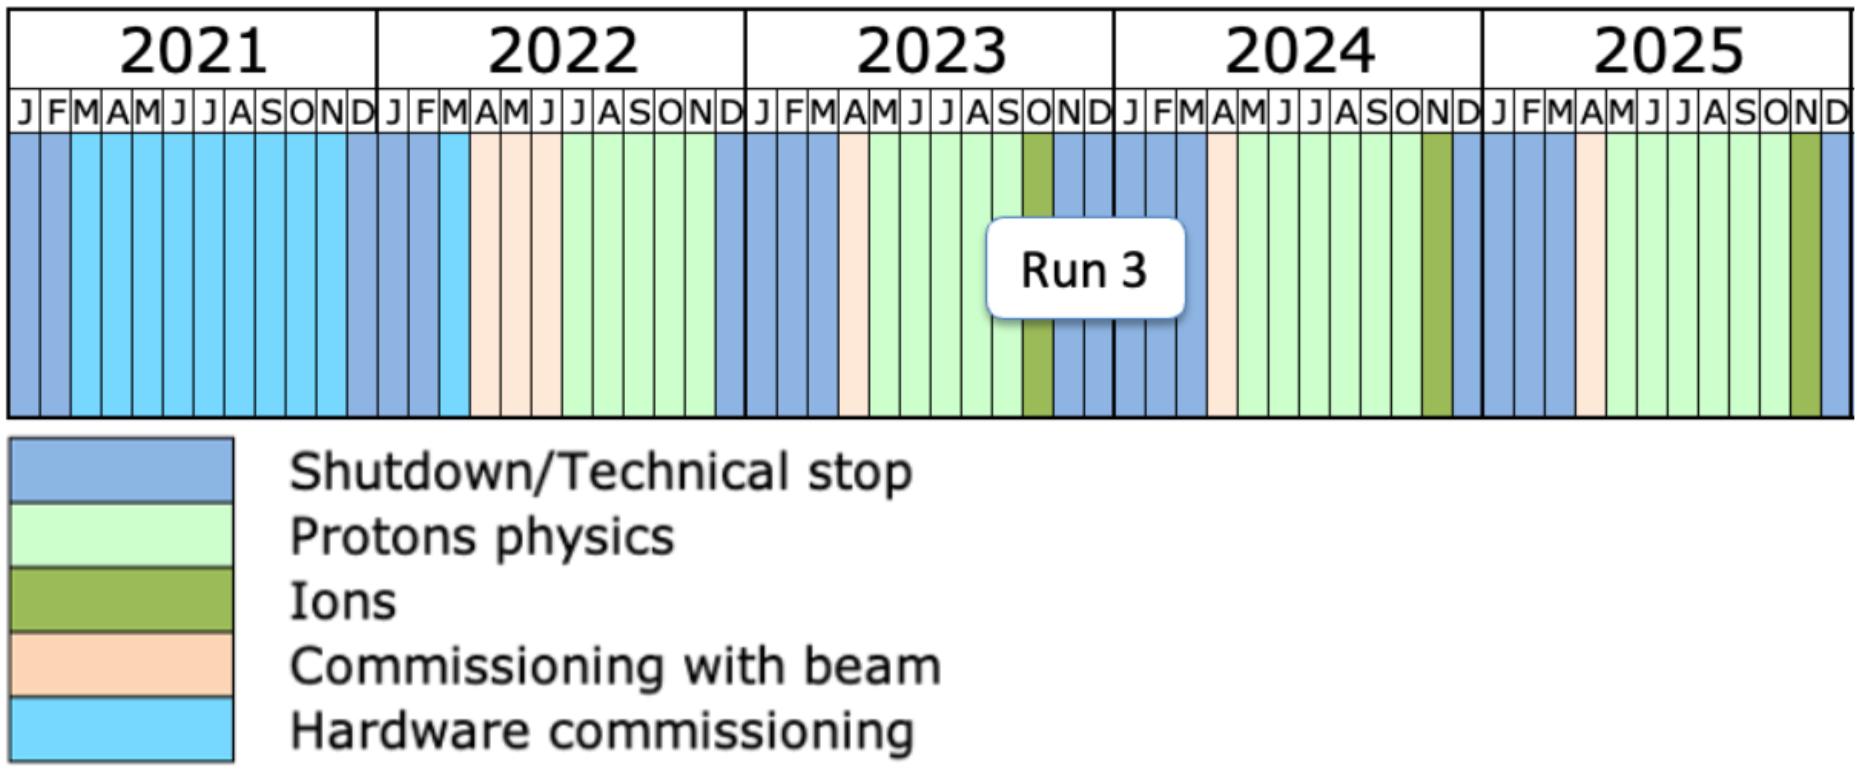
\includegraphics[width=0.8\textwidth]{images/assets/lhc_schedule.png}
    \caption[LHC Run 3 schedule]{The LHC schedule for Run 3, detailing the operational plan until 2024 (from \textit{Ref.} \cite{LHCSchedule}).}
    \label{fig:lhc_schedule}
\end{figure}

\subsection{Accelerator Complex}
\label{subsec:acc_complex}

\newacronym{bcid}{BCID}{Bunch Crossing Identifier}

The \acrshort{lhc} is only the final stage of a complex series of accelerators that prepare the particles for collision. Before protons are injected into the \acrshort{lhc}, they pass through a sequence of smaller accelerators that progressively increase their energy. This series of accelerators forms the comprehensive CERN accelerator complex, as shown in Figure~\ref{fig:cern_acc_complex}.

\begin{figure}[h]
	\centering
	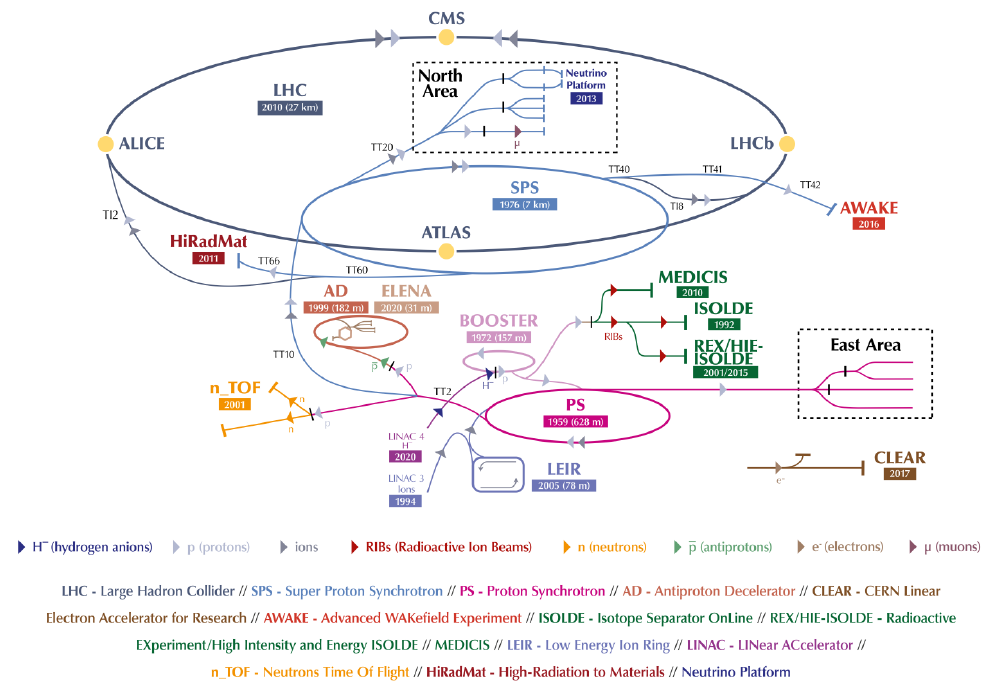
\includegraphics[width=\textwidth]{images/assets/cern_accelerator_complex.png}
	\caption[CERN Accelerator Sequence]{Diagram of the \acrshort{cern} Accelerator Sequence (from \textit{Ref.} \cite{cern-accelerator-complex}): Sequence of accelerators that prepare protons for injection into the \acrshort{lhc}. The path that protons follow can be traced from Linac4, to BOOSTER, to the PS, to the SPS, and finally to the LHC. Highlighed in yellow are the four main experiments at the \acrshort{lhc}. The LINAC3 and LEIR, whose purpose is to provide ions for the LHC, are also shown.}
	\label{fig:cern_acc_complex}
\end{figure}

The \acrshort{cern} accelerator complex begins its operations with the Linear Accelerator 4 (Linac4) \cite{Linac4}, which, since 2020, has served as the primary source for proton beams. Linac4 boosts the energy of negative hydrogen ions (H$^-$), hydrogen atoms with an additional electron, to 160 million MeV. Using radio frequency (RF) cavities, Linac4 charges a series of conductors in an alternating positive and negative manner, causing the particles to be accelerated. Before being pulsed through the accelerator, the H$^-$ ions are squeezed into a tight beam using quadrupole magnets. These ions are then readied to enter the Proton Synchrotron Booster (PSB), where they lose their two extra electrons and only the protons remain. The PSB further accelerates these protons to 2 GeV, before they proceed to the Proton Synchrotron (PS). At the PS, the proton energy is increased to 26 GeV. Subsequently, the protons are directed to the Super Proton Synchrotron (SPS), where their energy reaches 450 GeV. Finally, these protons are conveyed to the \acrshort{lhc}, where two beams are accelerated to a cumulative energy of 14 TeV.

In addition to protons, the \acrshort{lhc} also accelerates heavy ions, namely, lead and xenon cores. These ions initially enter the Linear Accelerator 3 (Linac3). Once gathered, they are sped up in the Low Energy Ion Ring (LEIR) and eventually follow the same trajectory as the protons to reach their maximum energy level.


\subsection{Particle Beams}
\label{subsec:particle_beams_lhc}

In the \acrshort{lhc}, particles are grouped into bunches, each containing approximately $10^{11}$ protons at the start of a physics fill. These bunches travel around a 27 km ring at nearly the speed of light, resulting in an orbiting frequency of approximately 11245.5 Hz. The RF cavities that accelerate the bunches operate with an oscillating electric field at a frequency of 400 MHz, creating a total of 35640 RF buckets, each spaced 2.5 ns apart. This arrangement is demanding, as it requires a high degree of resolution for any detector system aiming to obtain measurements per bucket. To alleviate this issue, buckets are grouped into sets of 10, with only the first bucket nominally filled with particles. This grouping increases the spacing between filled particle bunches to 25 ns. These bunch slots are referred to as bunch crossings and assigned a unique number called \acrfull{bcid}, ranging from 1 to 3564.

In each \acrshort{lhc} fill, a set of definitions known as a filling scheme is established. This scheme provides information on parameters such as the bunch spacing, the number of filled bunches per beam, the number of collisions at each \acrshort{ip}, and the maximum number of consecutive bunches, also known as a train, among others. The filling scheme heavily influences the physics conditions of the fill, dictating the experimental environment and collision dynamics. Special fills and given identified by a counter. may be requested to address a unique number that is incremented every time  experimental conditions in order to achieve the desired physics goals.


\subsection{Compact Muon Solenoid Experiment}
\label{subsec:cms}

The \acrlong{cms} \cite{TheCMSCollaboration_2008}, is a multi-purpose detector operating at the \acrshort{lhc}, designed to operate under high luminosity conditions. These conditions require radiation resistance, high granularity detectors and a carefully designed readout and trigger system. To fulfill its requirements the \acrshort{cms} apparatus is composed of a series of subsystems. Figure~\ref{fig:cms_detector} shows a schematic of the \acrshort{cms} detector and its subsystems. \acrshort{cms} is located underground close to the French village of Cessy, between Lake Geneva and the Jura mountains. It's coordinate system in relation to \acrshort{lhc}'s cilinder is ilustrate in Figure~\ref{fig:cms_system_coordinates}.

\begin{figure}[h]
	\centering
	\makebox[\textwidth][c]{%
		\begin{minipage}[b]{0.5\textwidth}
			\centering
			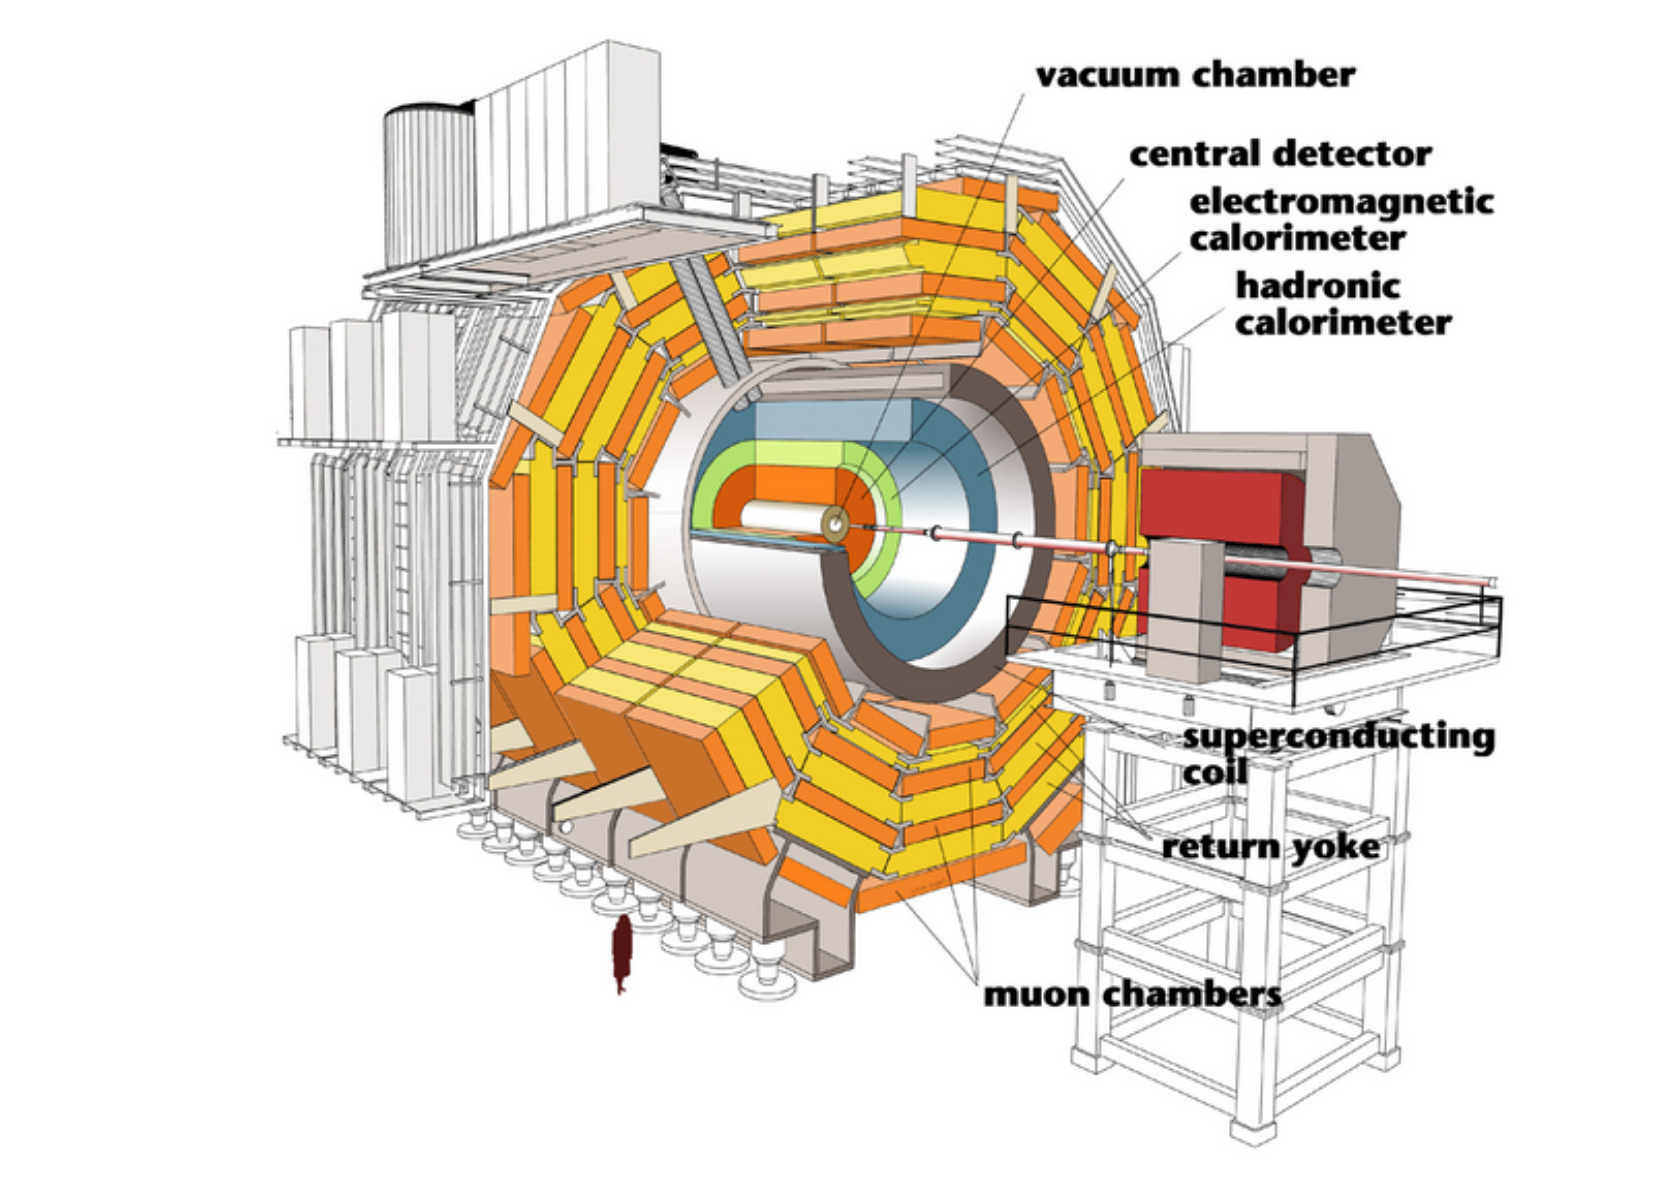
\includegraphics[width=\textwidth]{images/assets/cms_detector.png}
			\subcaption{}
			\label{fig:cms_detector}
		\end{minipage}
		\hspace{0.05\textwidth}
		\begin{minipage}[b]{0.5\textwidth}
			\centering
			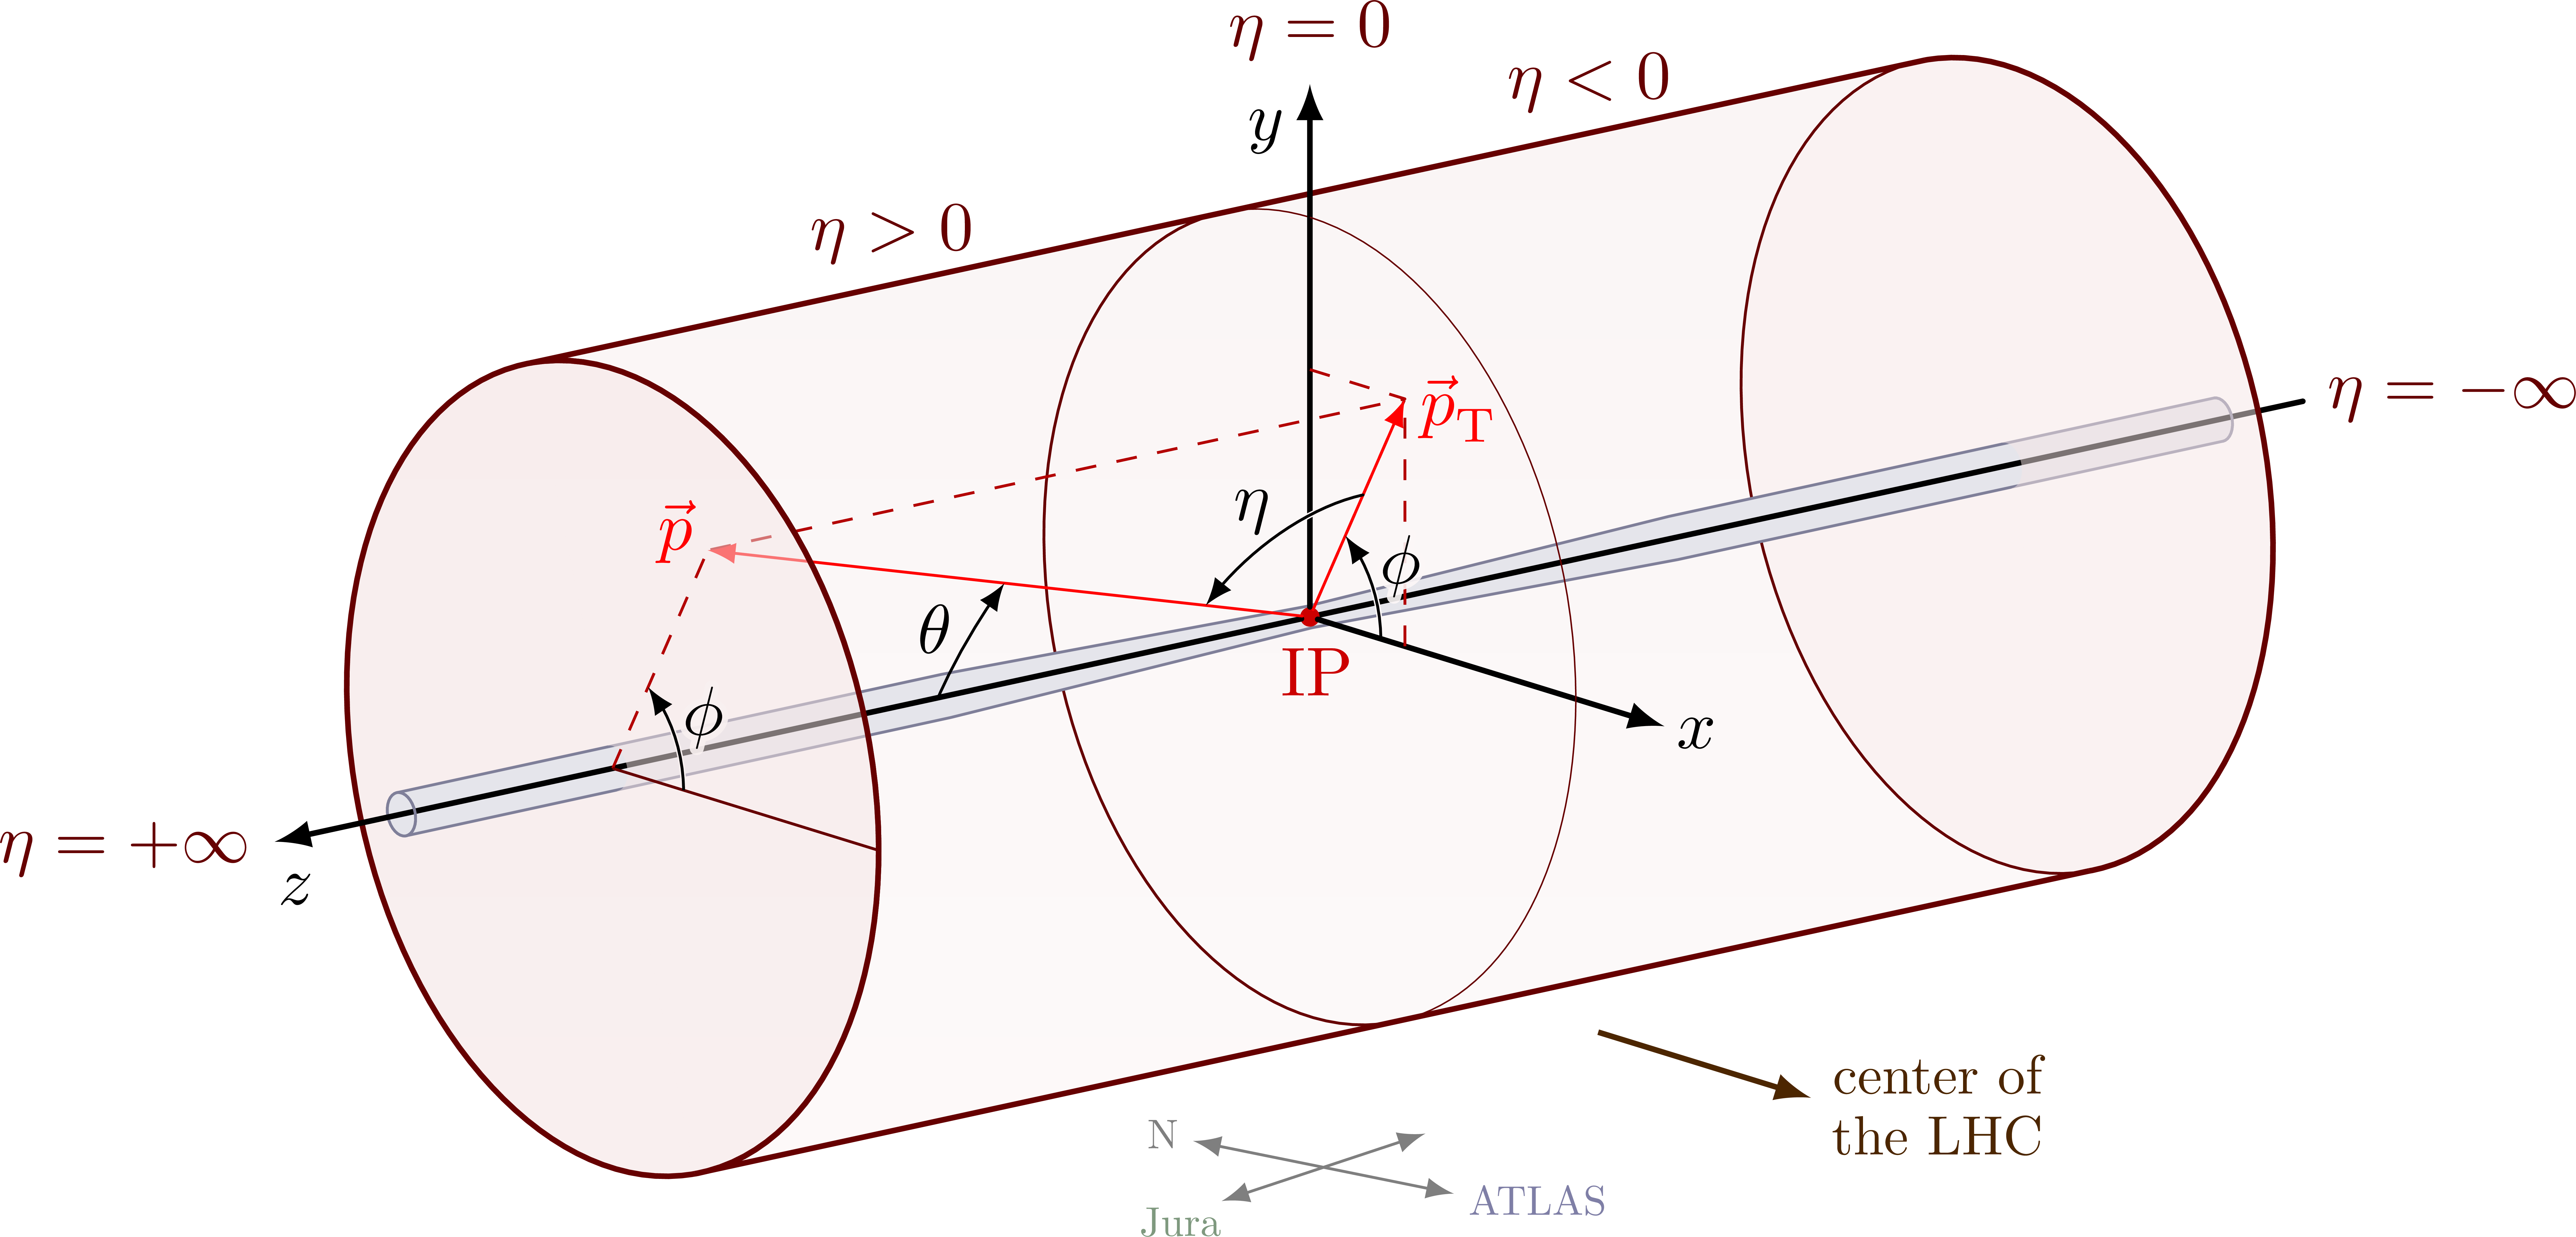
\includegraphics[width=\textwidth]{images/assets/cms_system_coordinates.pdf}
			\subcaption{}
			\label{fig:cms_system_coordinates}
		\end{minipage}
	}
	\caption[CMS detector and coordinate system]{(a) Schematic of the \acrshort{cms} detector outlining its subsystems (adapted from \textit{Ref.} \cite{CERN:39040}). (b) Diagram of the \acrshort{cms} coordinate system as seen with the \acrshort{lhc} cylinder in the background. The $x$-axis points radially to the center of the \acrshort{lhc} ring, the $y$-axis points upwards, and the $z$-axis points along the beam direction. The azimuthal angle, $\phi$, is measured from the $x$-axis to the $\vv{p}_T$ vector in the $xOy$ plane. The polar angle, $\theta$, is measured from the $z$-axis to the $\vv{p}$ vector. Each zone is labeled with the corresponding pseudorapidity, $\eta$, defined as $\eta = - \ln \tan (\theta / 2)$.}
	\label{fig:cms_images}
\end{figure}

As stated in Section~\ref{subsec:lhc}, the \acrshort{cms} physics program encompasses a wide range of topics. From the discovery of the Higgs boson, to continuosly probing the \acrshort{sm} throught precision measurements, to searching for new physics phenomena at high energy scales. The detector is built from the conjunction of multiple layers of subsystems, each with a dedicated focus on measuring specific subproducts of the collision events as they traverse the detector. The subsystems, from the center outwards, are depicted in Figure~\ref{fig:cms_slice}.

\begin{figure}[h]
	\centering
	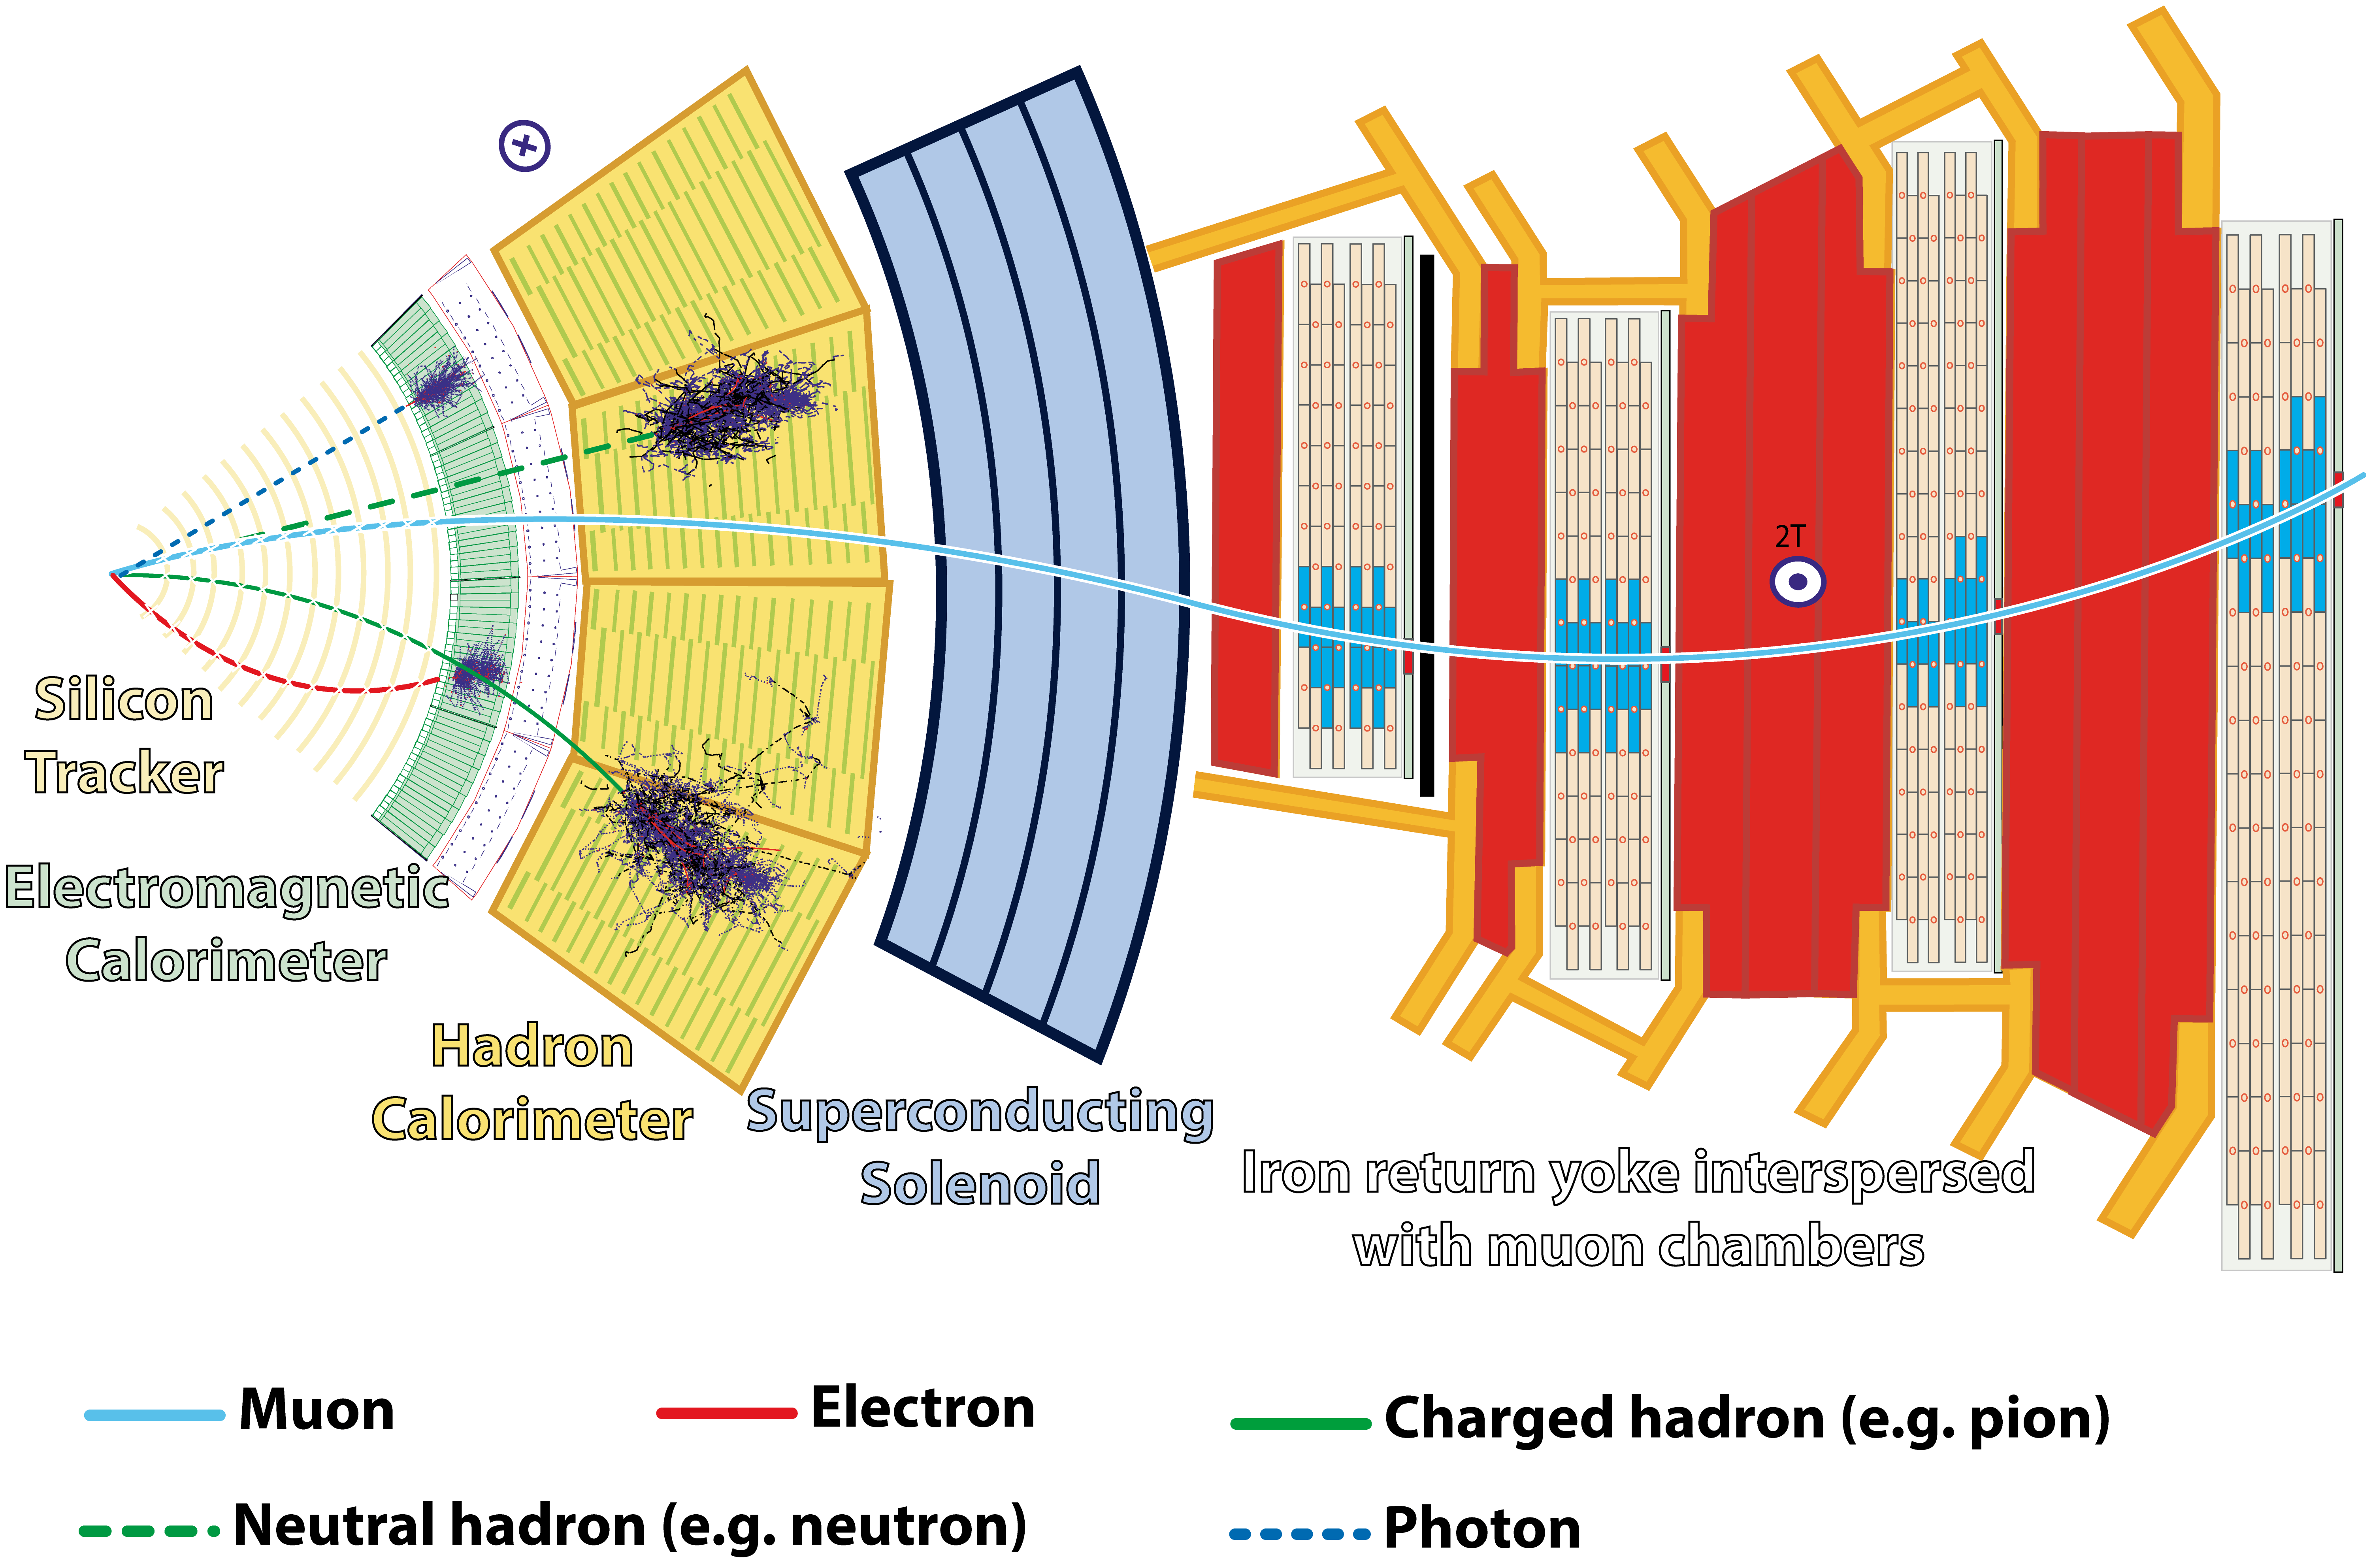
\includegraphics[width=\textwidth]{images/assets/cms_slice.png}
	\caption[Tranverse slice of CMS detector]{Transverse slice of the \acrshort{cms} detector (from \textit{Ref.} \cite{Barney:2120661}). The subsystems are shown from the center outwards: the silicon tracker, the electromagnetic calorimeter, the hadronic calorimeter, and the muon system.}
	\label{fig:cms_slice}
\end{figure}

\newacronym{ecal}{ECAL}{Electromagnetic Calorimeter}
\newacronym{hcal}{HCAL}{Hadronic Calorimeter}

The part of the detector closest to the beam pipe is the silicon tracker. This subsystem is composed of silicon sensors that track the paths of particles as they deposit charge while moving through it. Influenced by the \acrshort{cms} magnet, the curvature of these particles' paths provides crucial information for calculating their momentum, with more curved paths indicating lower momentum. The tracker can reconstruct the paths of electrons, hadrons, and high-energy muons. Immediately following the tracker are the \acrshort{cms} calorimeters: the \acrfull{ecal} and the \acrfull{hcal}. These calorimeters measure the energy of particles by stopping them and measuring the energy they deposit. The \acrshort{ecal}, composed of lead tungstate crystals, detects electrons and photons by scintillating upon interaction with these particles. Photodetectors, designed to operate within the high magnetic field, are attached to the back of each crystal to detect the scintillation light and convert it to an electrical signal that is then amplified and analyzed. The \acrshort{hcal} measures the energy of hadrons, which are particles made of quarks and gluons, such as protons and neutrons. Additionally, it allows for the indirect measurement of non-interacting particles, such as neutrinos, through the missing transverse energy, which represents the imbalance in the transverse momentum of the particles in the event. The \acrshort{hcal} is constructed with alternating layers of absorber and fluorescent materials, producing rapid light pulses when particles pass through. It is organized into several sections: the barrel (HB), outer barrel (HO), endcap (HE), and forward (HF) sections. Muons, heavy cousins of electrons, are the particles most likely to pass through the calorimeters and reach the muon system. The muon system is the outermost layer of the \acrshort{cms} detector and is designed to detect muons. It is composed of three types of detectors: Drift Tubes (DT), Cathode Strip Chambers (CSC), and Resistive Plate Chambers (RPC). Detailed information on \acrshort{cms} subsystems can be found in \cite{CERN-LHCC-2020-004}.

\section{Luminosity}
\label{sec:luminosity}

Luminosity is essential in particle physics research for two key reasons. First, accurate measurements of instantaneous luminosity are crucial for tracking the performance of both the accelerator and its associated detectors \cite{PhysRevAccelBeams.21.102801}. Second, integrated luminosity often represents the primary source of uncertainty in numerous cross-section measurements \cite{cms2022measurement, sirunyan2019measurement}. This section provides a detailed overview of the concept of luminosity.

\subsection{Instantaneous and Integrated Luminosity}
\newacronym{sbil}{SBIL}{Single Bunch Instantaneous Luminosity}

Luminosity is defined as the ratio between the rate of events, $R$, and the cross-section of a given process, $\sigma$, being studied:
\begin{equation}
    \label{eq:inst-luminosity}
    \mathcal{L} = \frac{R}{\sigma}
\end{equation}
$\mathcal{L}$ has then units of $[\mathrm{area}]^{-1} [\mathrm{time}]^{-1}$ where cm$^{-2}$s$^{-1}$ or fb$^{-1}$s$^{-1}$ are common units ($1$ barn  $= 10^{-28}$ m$^{-2}$). Integrating over a given time interval, $t_2 - t_1$, yields the integrated luminosity, $L$:
\begin{equation}
    \label{eq:int-luminosity}
    L = \int_{t_1}^{t_2} \mathcal{L} dt = \int_{t_1}^{t_2} \frac{R}{\sigma} dt = \frac{N}{\sigma}
\end{equation}
It follows that $L$ is proportional to the number of events, $N$, produced in the collider.

From \autoref{eq:int-luminosity} it can be seen that luminosity can be measured if the cross-section of a given process is known. This is the case for lepton colliders, where the ``candle" process $e^+ e^- \rightarrow e^+ e^-$ is used to measure luminosity \cite{Burkhardt:1056691}. However, for hadron colliders, which involve collisions of particles made of quarks, such as protons, this approach is not feasible due to the large uncertainties in the calculation of cross-sections. Another approach is to measure luminosity using machine parameters, as described in the next section.

\subsection{Luminosity from Machine Parameters}
\label{subsec:luminosity_from_machine_parameters}

The \acrfull{sbil}, $\mathcal{L}_b$, can be measured using the collider's machine parameters \cite{Burkhardt:1056691}.
\begin{figure}[h]
    \centering
    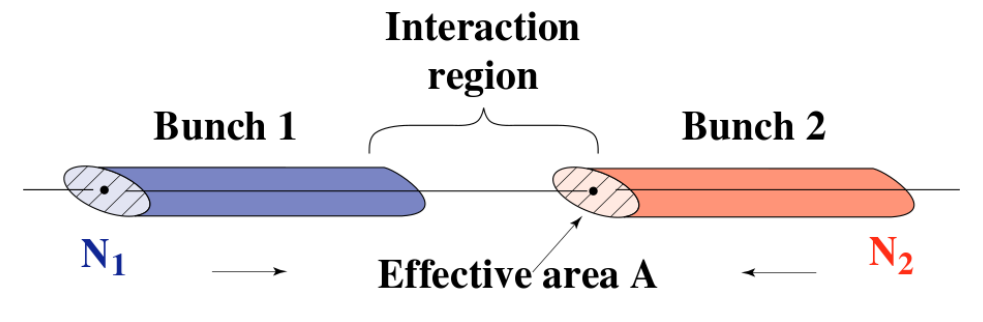
\includegraphics[width=0.8\textwidth]{images/assets/bunch_crossing.png}
    \caption[Bunch crossing illustration]{Bunch crossing ilustration (from \textit{Ref.} \cite{Burkhardt:1056691}).}
    \label{fig:bunch_crossing}
\end{figure}
For colliding bunches containing $N_1$ and $N_2$ particles respectively, the expected value of $\mathcal{L}_b$ is given by the following equation:
\begin{equation}
    \label{eq:sbil-machine-params}
    \mathcal{L}_b = \frac{N_1 N_2 f_{rev}}{A_{eff}}
\end{equation}
In this equation, $f_{rev}$ represents the orbiting frequency around the \acrshort{lhc}, as described in \autoref{subsec:particle_beams_lhc}, and $A_{eff}$ is the effective transverse area where collisions occur, also refered to as the luminous region. If the transverse distribution of particles was normal, $A_{eff}$ would be equivalent to the transverse bunch overlap. However, considering the transverse particle distributions $\rho_1$ for bunch 1 and $\rho_2$ for bunch 2, the effective transverse area is defined by the overlap integral:
\begin{equation}
    \label{eq:effective-area}
    \frac{1}{A_{eff}} = 2 \int \rho_1(x,y) \rho_2(x,y) dxdy
\end{equation}
The factor of 2 is the Møller factor, which accounts for the fact that the two bunches are colliding at equal relativistic speeds and in opposite directions \cite{furman2003moeller}. Typically, it's assumed that these transverse particle distributions are uncoupled, meaning: 
\begin{equation}
    \begin{cases}
		\rho_1 \left(x, y \right) = \rho_{1x} \left( x \right) \rho_{1y} \left( y \right) \\
		\rho_2 \left(x, y \right) = \rho_{2x} \left( x \right) \rho_{2y} \left( y \right) \\
    \end{cases}\,.
\end{equation}
Under this assumption, the effective transverse area can be rewritten as:
\begin{equation}
    \label{eq:effective-area}
    \frac{1}{A_{eff}} = 2 \int \rho_{1x}(x) \rho_{2x}(x) dx \times \int \rho_{1y}(y) \rho_{2y}(y) dy = \frac{1}{W_{eff}} \times \frac{1}{H_{eff}}
\end{equation}
Here, $W_{eff}$ and $H_{eff}$ represent the effective transverse width and height, respectively. Substituting this back into equation \ref{eq:sbil-machine-params}, we get:
\begin{equation}
    \label{eq:sbil-machine-params-2}
    \mathcal{L}_b = 2 N_1 N_2 f_{rev} \int \rho_{1x}(x) \rho_{2x}(x) dx \times \int \rho_{1y}(y) \rho_{2y}(y) dy
\end{equation}
Further assuming Gaussian transverse particle distributions with widths $\sigma_{x1}$, $\sigma_{x2}$ and heights $\sigma_{y1}$, $\sigma_{y2}$, the equation becomes:
\begin{equation}
    \label{eq:sbil-machine-params-3}
    \mathcal{L}_b = 2 N_1 N_2 f_{rev} \int G_x (\sigma_{x1}) G_x (\sigma_{x2}) dx \times \int G_y (\sigma_{y1}) G_y (\sigma_{y2}) dy
\end{equation}
$G_i (\sigma)$ in this context is the Gaussian distribution with standard deviation $\sigma$ in the $i \in {x,y}$ direction and a mean of zero:
\begin{equation}
    \label{eq:gaussian-distribution}
    G_i (\sigma) = \frac{1}{\sigma \sqrt{2 \pi}} e^{-\frac{i^2}{2 \sigma^2}}
\end{equation}
Expanding the first integral:
\begin{equation}
	\label{eq:sbil-machine-params-4}
	\int G_x (\sigma_{x1}) G_x (\sigma_{x2}) dx = \frac{1}{2 \pi \sigma_{x1} \sigma_{x2}} \int e^{-\frac{x^2 \left( \sigma_{x1}^2 + \sigma_{x2}^2 \right)}{2 \sigma_{x1}^2 \sigma_{x2}^2}} dx
\end{equation}
and considering
\begin{equation}
	\int e^{-a x^2} dx = \sqrt{\frac{\pi}{2a}}
\end{equation}
equation \ref{eq:sbil-machine-params-4} can be simplified to:
\begin{equation}
	\label{eq:sbil-machine-params-5}
	\int G_x (\sigma_{x1}) G_x (\sigma_{x2}) dx = \frac{1}{2 \pi \sigma_{x1} \sigma_{x2}} \sqrt {\frac{\pi \sigma_{x1}^2 \sigma_{x2}^2}{\sigma_{x1}^2 + \sigma_{x2}^2}} = \frac{1}{2 \sqrt{\pi} \sqrt{\sigma_{x1}^2 + \sigma_{x2}^2}}
\end{equation}
Using the same approach for the second integral and plugin the results back into equation \ref{eq:sbil-machine-params-3} we get: 
\begin{equation}
\label{eq:sbil-machine-params-6}
\mathcal{L}_b = \frac{N_1 N_2 f_{rev}}{2 \pi \Sigma_X \Sigma_Y}
\end{equation}
where $\Sigma_X = \sqrt{2\pi} W_{eff} = \sqrt{2\pi} \sqrt{\sigma_{x1}^2 + \sigma_{x2}^2}$ and $\Sigma_Y = \sqrt{2\pi} H_{eff} = \sqrt{2\pi} \sqrt{\sigma_{y1}^2 + \sigma_{y2}^2}$. In the case of round beams, the RMS widths of the horizontal and vertical beam profiles are equivalent to $\sqrt{\epsilon_{N} \beta^{*} / \gamma}$. $\gamma$ is the relativistic Lorentz factor, and $\beta^{*}$ corresponds to the value of the optical function $\beta$ at the IP. $\epsilon_{N}$ is the normalized transverse emittance, valued at $3.75\mu m$ for the LHC \cite{Brüning:782076}.

\subsection{Luminosity Calibration}
\label{subsec:luminosity_calibration}

Luminosity detectors, also called luminometers, are located at the IPs of the LHC and measure the observable quantities of the collisions. Due to the differences between the luminometers, the nature of their recorded observables and their location at the \acrshort{cms} cavern, each is assumed to only capture a fraction of the total collisions. This bias in the luminometers is accounted for by a detector-specific calibration factor, the visible cross-section, $\sigma_{vis}$. Using equations \ref{eq:inst-luminosity} and \ref{eq:sbil-machine-params-3} this calibration can be expressed as:
\begin{equation}
    \label{eq:vis-cross-section}
    \sigma_{vis} = \frac{2 \pi \Sigma_X \Sigma_Y R}{N_1 N_2 f_{rev}}
\end{equation}
Once calculated, the visible cross-section can be used to convert the measured rates to luminosity:
\begin{equation}
    \label{eq:luminosity-from-rates}
    \mathcal{L} = \frac{R}{\sigma_{vis}}
\end{equation}
In both these equations, $R$ represents the measured rate of events from a particular luminometer.

\subsection{Zero Counting Method}
\label{subsec:zero-counting}

Due to the constraints in the read-out electronics of the luminometers, there's a chance that simultaneous particle hits might be recorded as a single event. This necessitates a more advanced approach to counting hits accurately. It is postulated that the distribution of the number of hits can be modeled by a Poisson distribution \cite{TheLHCbcollaboration_2014} with mean, $\mu$, that is proportional to luminosity.
\begin{equation}
    \label{eq:luminosity-from-hits}
    \mathcal{L}_b = \frac{\mu f_{rev}}{\sigma}
\end{equation}
The zero-counting method is based on this assumption. It consists of calculating the probability that a luminometer records zero hits, $P_0$, regardless of the number of collisions that occur. This probability is given by the following equation:
\begin{equation}
    \label{eq:zero-counting}
    P_0 = \sum_{i=0}^{\infty} \frac{\mu^i e^{-\mu}}{i!} p^i = e^{-\mu(1-p)}
\end{equation}
$\mu$ is the mean number of hits per bunch crossing, also known as pileup, and $p$ is the probability that no observables are recorded in a bunch crossing with $i$ interactions. It then follows that luminosity is proportional to the natural logarithm of $P_0$:
\begin{equation}
    \label{eq:luminosity-from-hits-2}
    \mathcal{L}_b = \frac{\mu f_{rev}}{\sigma} = - \frac{\log (P_0)}{1-p} \frac{f_{rev}}{\sigma} = - \log (P_0) \frac{f_{rev}}{\sigma_{\mathrm{vis}}}
\end{equation}
The value of $p$ is here absorbed into the visible cross section \cite{Sirunyan:2759951} and does not need to be known beforehand.

The zero counting method is not without its limitations. from \autoref{eq:zero-counting} it can be seen that the probability of recording zero hits decreases exponentially with increasing pileup, or similarly, increasing luminosity. This leads to a phenomenon known as zero starvation, where the probability of recording zero hits, $P_0$, becomes very small. This can lead to a situation where the luminometer underestimates the number of hits, and consequently, the luminosity.

%%%%%%%%%%%%%%%%%%%%%%%%%%%%%%%%%%%%%%%%%%%%%%%%%%%%%%%%%%%%%%%%%
%% LUMINOMENTER: TO APPROACH AFTER KNOWING WHAT LUMINOISITY IS %%
%%%%%%%%%%%%%%%%%%%%%%%%%%%%%%%%%%%%%%%%%%%%%%%%%%%%%%%%%%%%%%%%%

\section{Luminometers}
\label{subsec:luminosity_detectors}

\newacronym{bril}{BRIL}{Beam Radiation Instrumentation and Luminosity}
\newacronym{plt}{PLT}{Pixel Luminosity Telescope}
\newacronym{bcm1f}{BCM1F}{Fast Beam Conditions Monitor}
\newacronym{4nb}{4NB}{4Nibble}
\newacronym{ls}{LS}{Lumisection}
\newacronym{bib}{BIB}{Beam-Induced Background}


The \acrfull{bril} group is responsible for measuring luminosity at \acrshort{cms}. In addition to this primary task, the group monitors \acrfull{bib} and dangerous beam loss events that may trigger a beam abort. They also manage beam timing, minimum bias triggers for data acquisition, and the monitoring and simulation of the radiation environment within the \acrshort{cms} cavern. Luminosity measurements are done with the use of dedicated detectors called luminometers.

These specialized detectors, are capable of providing luminosity measurements with a per-bunch spacial-granularity. At CMS, the number of events measured by most of these systems are integrated over $2^{14}$ \acrshort{lhc} orbits which accounts for $\approx 1.458s$. This ammount of time is refered to as a \acrfull{4nb}. Another interval of integration often used during luminosity analysis is the \acrfull{ls} and corresponds to 16 \acrshort{4nb}.

Since these detectors usually operate during long periods of time, four integers are used to select a particular operation period. These integers correspond to: a fill number, synchronized across all \acrshort{lhc} experiments; a run number, incremented every few hours and multiple times in a fill; a \acrshort{ls} number, unique to \acrshort{cms} and resetting every run; and a \acrshort{4nb}, also unique to \acrshort{cms} and resetting every lumisection. Most often than not, only a a pair of run and \acrshort{ls} numbers are used during analysis.

Figure~\ref{fig:cms_bril_detectors} shows the \acrshort{cms} location of all the systems operated by the \acrshort{bril} group.

\begin{figure}[h]
	\centering
	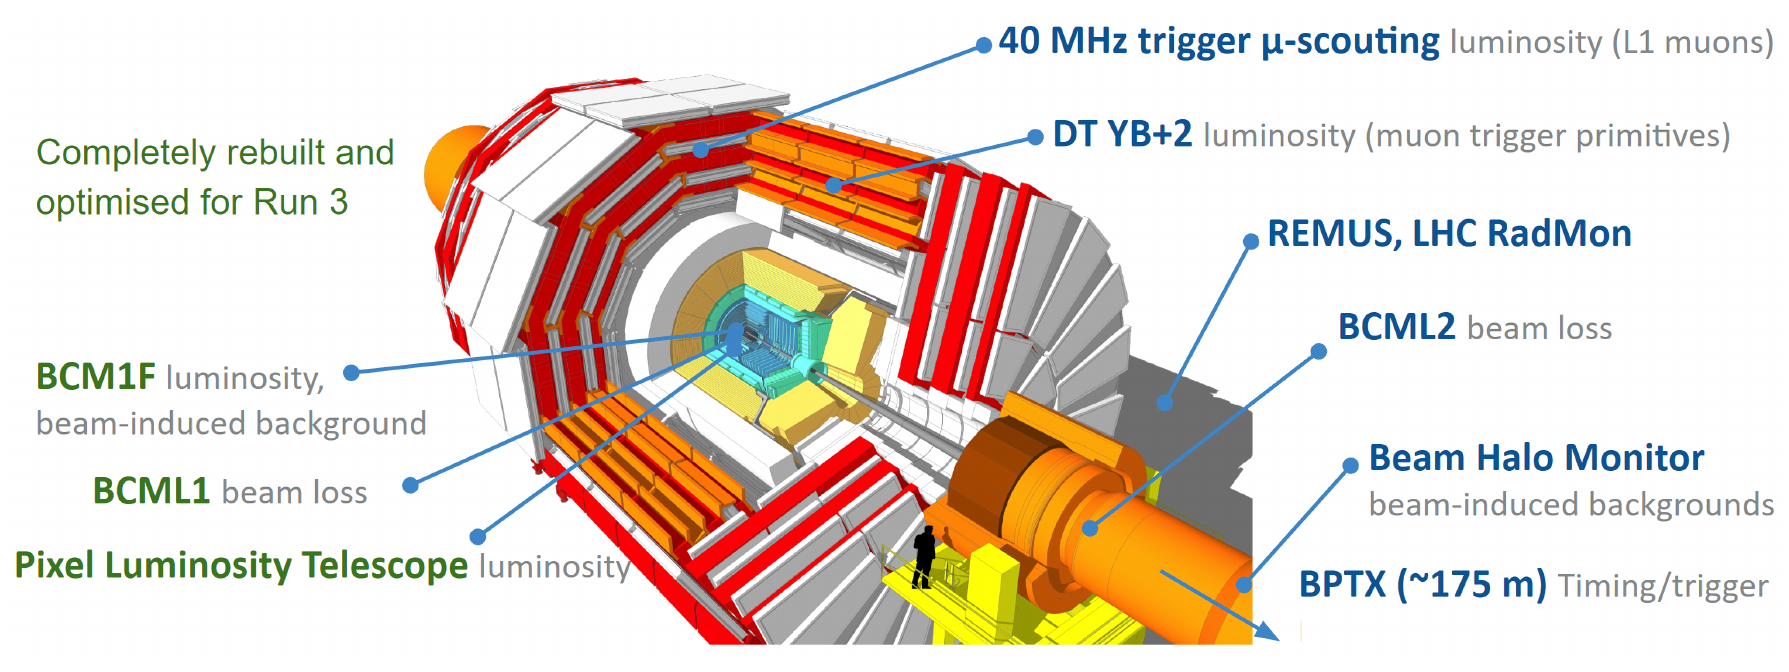
\includegraphics[width=\textwidth]{images/assets/cms_bril_detectors.png}
	\caption[BRIL systems at CMS]{Systems operated by BRIL group at the Compact Muon Solenoid experiment.Green text indicates, that the instrumentation has been rebuilt for Run 3 (from \textit{Ref.} \cite{Saariokari:2826125}).}
	\label{fig:cms_bril_detectors}
\end{figure}

For a detector to be used as a luminometer, it must meet certain essential requirements. One of the most critical use cases for luminometers is their ability to provide online instantaneous luminosity measurements. This capability is crucial as the for the operation of the LHC and the goals of the \acrshort{cms} experiment. Additionally, having per-bunch granularity is important, as the calibration process for the luminometers heavily depends on the available statistics, as will be addressed in \autoref{subsec:the_van_der_meer_scan_methodology}.

Two other characteristics of paramount importance are the stability of the detector over long periods of time and the detector’s response to varying experimental conditions. The former is necessary to ensure that the luminometers can provide reliable measurements throughout the entire year of operations. A luminometer’s stability is typically affected by prolonged exposure to radiation, which decreases the detector’s efficiency and results in a decrease in its reported luminosity over the course of the year. In order to adjust the detector’s response, several adjustments are made to the detector’s operating conditions. It is important to understand that these corrective procedures do not improve the detectors performance but only normalize it to its original and optimal state.

The latter characteristic concerns how the detector’s response changes under different experimental conditions. Initially, as we approach stable beam conditions in a fill, the pileup is at its highest. As the fill progresses, the natural decay of the beam population, commonly referred to as burn-off, causes the pileup to decrease. A luminometer’s response to these changes in pileup conditions must be as linear as possible with respect to luminosity. Additionally, changes in the filling scheme can affect the detector’s response, as some detectors are more sensitive to afterglow effects, where the signal from a previous bunch crossing is still present in the immediately adjacent bunch crossings. Similar to maintaining the detector's stability, the linearity of the luminometer’s response is preserved through corrective procedures, which will be discussed in \autoref{subsec:extrapolation_of_vdM_calibration} and with focus on 2023 data in \autoref{ch:2023_luminosity_calibration}.

The following subsections will describe the luminometers that were considered for this work, their positions at the LHC and how the luminosity is extracted from their observable measurements.

\subsection{Hadron Forward}
\newacronym{hf}{HF}{Hadron Forward}
\newacronym{hfoc}{HFOC}{Hadron Forward Occupancy Count}
\newacronym{hfet}{HFET}{Hadron Forward Transverse Energy}

As stated in \autoref{subsec:cms}, the \acrshort{cms} \acrshort{hcal} is composed of several sections, one of which is the \acrfull{hf} calorimeter \cite{CMS:2012tda}. The \acrshort{hf} is constructed from quartz scintillators embedded in steel absorbers and is located at $z \pm 11.2$m from the \acrshort{ip}, covering a pseudorapidity range of $3 < |\eta| < 5$. This range allows for better detection of missing transverse energy, which is crucial for probing the \acrshort{sm} and searching for new physics phenomena.

The \acrshort{hf} calorimeter uses Photomultiplier Tubes (PMTs) to collect Cherenkov light produced by particles passing through the quartz scintillators. A dedicated readout system collects these signals and converts them into luminosity measurements using two methods. The original \acrshort{hfoc} method tracks the fraction of bunch crossings with no energy deposition above a threshold in specific \acrshort{hf} towers (eta rings 31 and 32). The average number of these counts, $\mu$, is then converted to luminosity via the zero-counting method.

A second method, the \acrshort{hfet} method, was implemented in 2016. It is based on the assumption that the measured transverse energy sum is proportional to the luminosity. This assumption is used to estimate the number of passing particles and convert it to luminosity. The HFET method is used in parallel with the HFOC method to cross-check the luminosity measurements.

\subsection{The Pixel Luminosity Telescope}
\label{subsubsec:plt}

One of the dedicated luminosity detectors is the \acrfull{plt} \cite{CMS-DP-2021-020}. This detector is based on the use of silicon pixel sensors, 48 in total, arranged in groups of 3 in a telescope-like structure. The sensors are placed at a distance of $1.75$m from both ends of the \acrshort{ip} at a $|\eta| \approx 4.2$, nearly parallel to the beam line. Figure~\ref{fig:cms_plt} shows the a diagram for the 48 sensors and the half of the detector with the mounting support.

\begin{figure}[H]
	\centering
	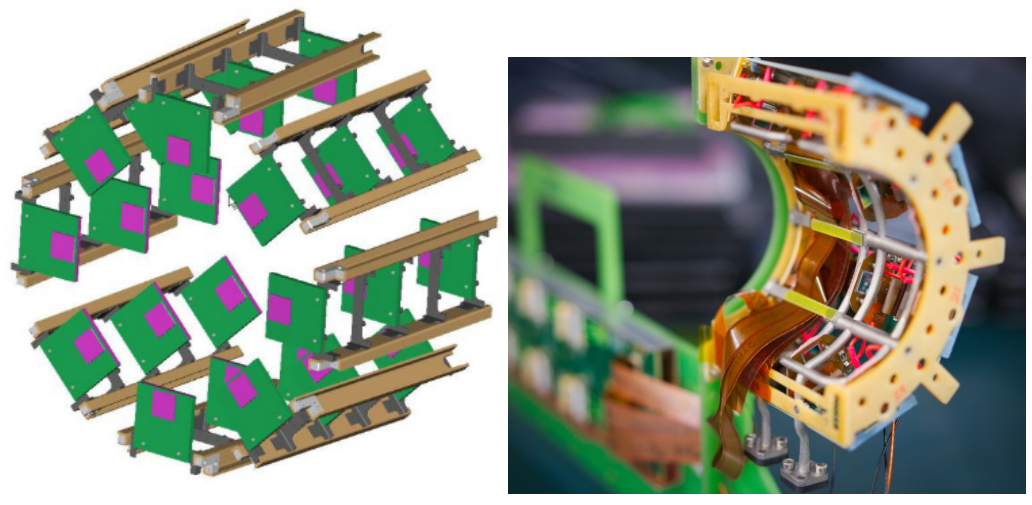
\includegraphics[width=\textwidth]{images/assets/cms_plt.png}
	\caption[PLT detector telescopes]{\textbf{Left}: Picture illustrating eight telescopes of the \acrshort{plt} detector, which correspond to half detector (from \textit{Ref.} \cite{Romeo:2797807}). \textbf{Right}: Half of the full \acrshort{plt} detector with mounting support and with visible connections to the readout electronic (from \textit{Ref.} \cite{DelannoySotomayor:2765247}).}
	\label{fig:cms_plt}
\end{figure}

\acrshort{plt}'s silicon sensors are bump bonded to PSI46v2 readout chip \cite{KASTLI2006188}, which offer two readout modes: the "fast-or" mode allows for a readout rate of 40MH$z$, allowing per bunch measurements. The full pixel data readout mode reads at a lower rate of 3.3 kH$z$ being usefull for other studies. A \acrshort{plt} "hit" is considered when a particle passes through the 3 sensors of a telescope, refered to as a triple coincidence. This method allows for track reconstruction which helps descern between particles from the collision and background noise. Figure~\ref{fig:plt_triple_coincidence} shows an illustration of a triple coincidence.

\begin{figure}[H]
	\centering
	\includegraphics[width=0.5\textwidth]{images/assets/TripleCoincidenceSketch.pdf}
	\caption[Triple coincidence in PLT]{Illustration of a triple coincidence in the \acrshort{plt} detector. A hit is considered when a particle passes through the 3 sensors of a telescope (from \textit{Ref.} \cite{Lujan:2797692}).}
	\label{fig:plt_triple_coincidence}
\end{figure}

The zero counting method, described in \autoref{subsec:zero-counting}, is used to convert the number of hits to luminosity. For PLT, the zero starvation effect is usually not a problem, as the tipical PLT occupancy is on the order 0.1-0.2 triple coincidences per telescope per bunch crossing at high luminosity conditions.

\subsection{The Fast Beam Conditions Monitor}

The \acrfull{bcm1f} \cite{CMS-DP-2022-033} can measure not only the luminosity but also the \acrshort{bib}. It consists of 24 silicon sensors arranged in four semi-circles, referred to as C-shapes, positioned 7.2 cm from the beam pipe and at a distance of 1.8 m on either side of the \acrshort{ip}. This placement allows for the separation of incoming and outgoing particles, corresponding to a flight time of 6.25 ns for particles traveling at relativistic speeds. This setup enables the discernment of signals originating from collisions, \acrshort{bib}, and noise caused by the activation of surrounding material \cite{Zagozdzinska_2016}. \autoref{fig:bcm1f_real_life} shows the arrangement of one of the C-shapes.

\begin{figure}[h]
\centering
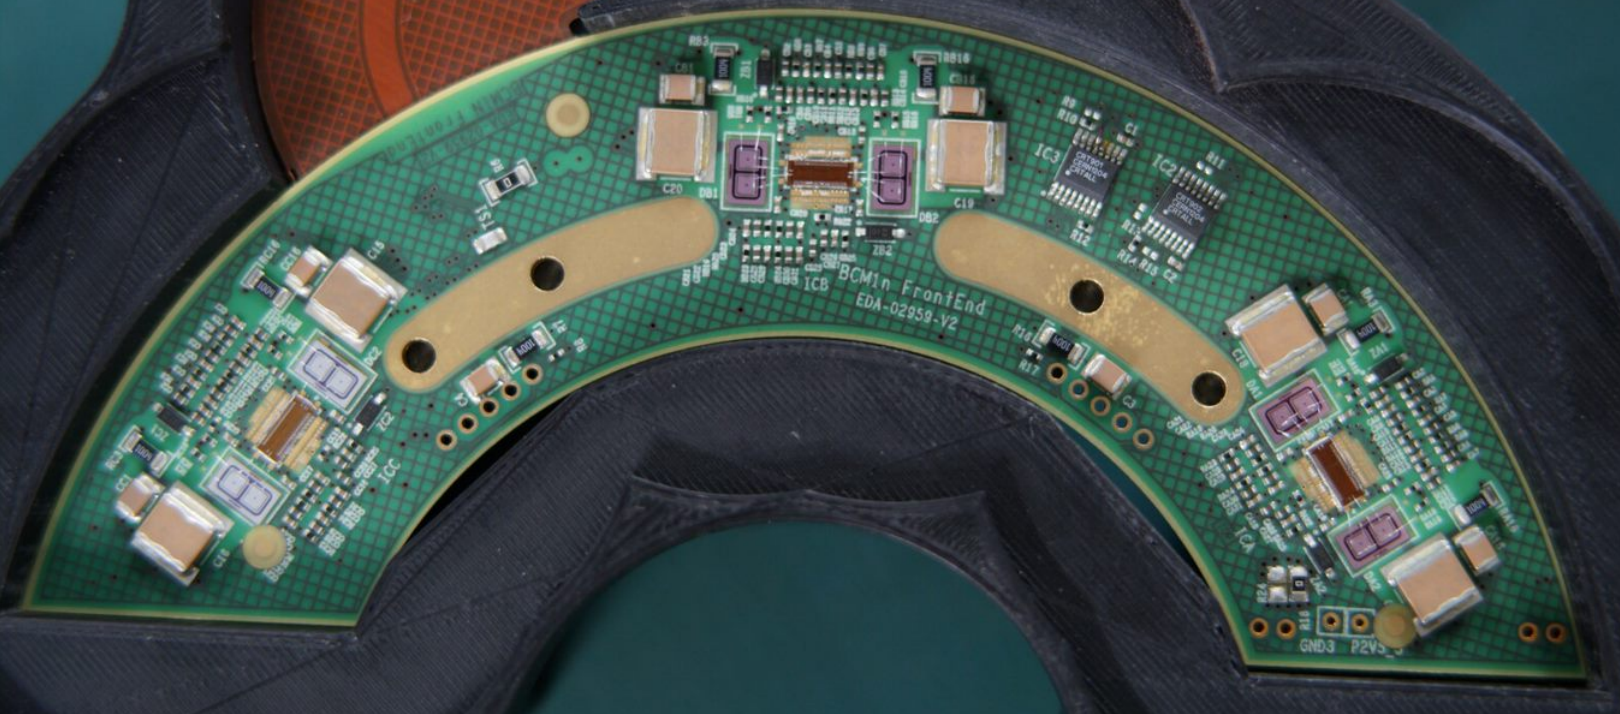
\includegraphics[width=\textwidth]{images/assets/bcm1f_real_life.png}
\caption[BCM1F sensor arrangement]{Arrangement of the six sensors in one of the C-shapes of the \acrshort{bcm1f} detector (from \textit{Ref.} \cite{DelannoySotomayor:2809025}).}
\label{fig:bcm1f_real_life}
\end{figure}

\newacronym{vme}{VME}{Versa Module Europa}
\newacronym{rhu}{RHU}{Realtime Histograming Unit}

A particle passing through the bulk of a silicon sensor will ionize the material, creating electron-hole pairs. These pairs are then separated by an electric field, generating a current pulse proportional to the energy of the particle. The signals detected in the sensors are read by two parallel systems. The older back-end system utilizes the \acrfull{vme} standard and was the primary system during Run 2. The newer $\mu$TCA-based system began operation in Run 3 \cite{Karacheban:2294183}.

The \acrshort{vme} back-end system discriminates signals using a constant threshold, and the hits are sent to a \acrfull{rhu}. The hits per bunch are then converted to luminosity using the zero-counting method. The $\mu$TCA system employs a more sophisticated approach, using a peak-finding algorithm that counts pulses based on the signal's derivative and amplitude. This method not only allows for more accurate distinction between hits and noise but also enables the detection of simultaneous hits by analyzing the pulse shape. Both systems, BCM1F and BCM1FUTCA, are used as independent luminometers.

\subsection{Pixel Cluster Counting}

The \acrshort{cms} Pixel detector is also used as a luminometer. Upgraded for Phase I, it consists of four barrel layer, BPIX, and three disks, FPIX, on each side of the \acrshort{ip} at distances of 291, 396, and 516 mm, respectively. The BPIX is made up of a total of 79 million pixels in 1184 modules, while the FPIX contains 45 million pixels in 672 modules. The layouts of the two detectors, the original and the upgraded one, are compared in \autoref{fig:pcc_layout}. Further details on the desing and construction of the upgraded Pixel detector can be found in \cite{tracker2020cms}.

\begin{figure}[h]
\centering
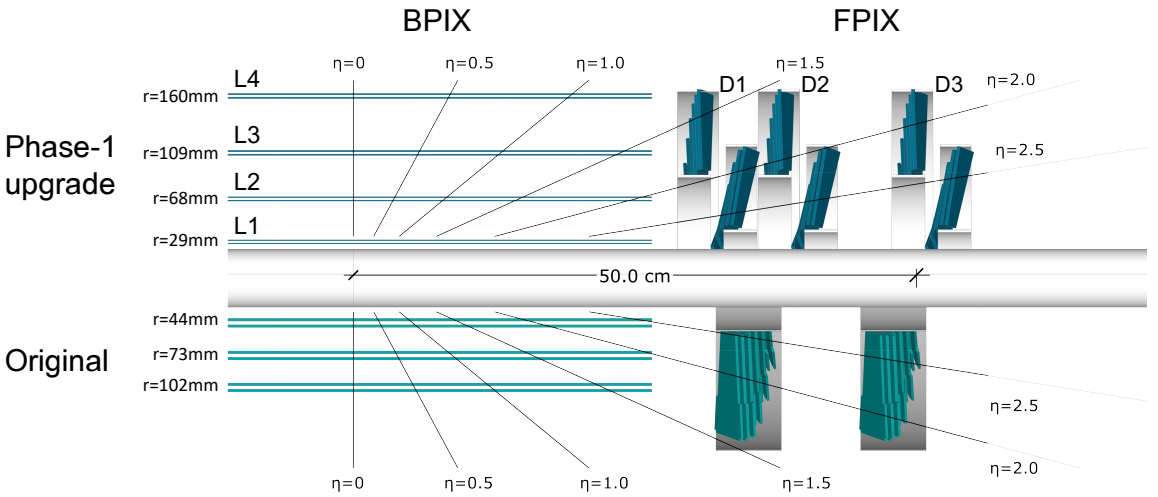
\includegraphics[width=\textwidth]{images/assets/pcc_upgrade.png}
\caption[Upgraded pixel detector]{Longitudinal view of the Phase 1-upgraded pixel detector compared to the original detector layout (from \textit{Ref.} \cite{tracker2020cms}). Labels L1 to L4 indicate the barrel layers, while D1 to D3 indicate the disks.}
\label{fig:pcc_layout}
\end{figure}

The Pixel Cluster Counting (PCC) method counts the mean number of clusters, a conglomerate amount of charged particle hits, in the pixel detector in zero bias events. The mean number of clusters, averaged over several measurements, can be expressed as

\begin{equation}
	\label{eq:pcc-clusters-mean}
	\langle N_{\text{clusters}} \rangle = \langle N_{\text{clusters} / \text{interaction}} \rangle \cdot \frac{\sigma_{\text{minBias}}}{f_{rev}} \cdot \mathcal{L}_b
\end{equation}

from which the PCC calibration factor can be calculated as $\sigma_{\text{vis}} = \sigma_{\text{minBias}} \cdot \langle N_{\text{clusters} / \text{interaction}} \rangle$ where $\sigma_{\text{minBias}}$ is the proton-proton cross section for minimum bias events. The $\langle N_{\text{clusters}} \rangle$ is measured by averaging the number of clusters over 23 second intervals with a 0.1\% statistical uncertainty for orbit integrated luminosity.

Due the large ammount of pixel systems, the PCC method has been shown to provide stable and linear luminosity measurements and was used as the primary luminometer for the \acrshort{cms} experiment in previous years \cite{Sirunyan:2759951}. The measurements from this detector are only used during the offline analysis. 

\subsection{Drift Tube}
\label{subsec:dt}

Located in the \acrshort{cms} muon system, the Drift Tube (DT) is a sub-system of the muon barrel (MB) that provides estimates the number of muon tracks passing through the detector. This estimation, done with the Barrel Muon Track Finder (BMTF) algorithm \cite{Triossi_2017}, is assumed to be proportional to the luminosity which allos for DT to be used as a luminometer. However, does not provide luminosity measurements with per bunch granularity, but rather \acrshort{ls}-integrated. This limitations makes measuring it's calibration factor, $\sigma_{\text{vis}}$, dependent on the other luminometers. However, due to its good stability and linearity, it is often calibrated to match other luminometers as a way to compare for stability and linearity.

%%%%%%%%%%%%%%%%%%%%%%%%%%%%%%%%%%%%%%%%%%%%%%%%%%%%%%%%%%%%%%%%%
%% LUMINOMENTER: TO APPROACH AFTER KNOWING WHAT LUMINOISITY IS %%
%%%%%%%%%%%%%%%%%%%%%%%%%%%%%%%%%%%%%%%%%%%%%%%%%%%%%%%%%%%%%%%%%

\chapter{State of the Art}

CERN’s mission of understanding the fundamental structure of the universe is heavily reliant on particle accelerators. The effectiveness of the experiments conducted in these machines is closely tied to their luminosity, as detailed in \autoref{sec:luminosity}. In this chapter I will begin by explaining the Van der Meer (vdM) scan methodology used to measure the luminometer's calibration factor. Subsequently, I'll discuss the corrective procedures that are applied in order to enhance the accuracy and precision of this method. Finally, I will address the challenges associated with extrapolating the results obtained with the vdM method for the rest of the data taking year. Through this discussion, I hope to emphasize the complexities and challenges associated with reporting accurate luminosity measurements at high pileup.

\section{Absolute luminosity calibration}
\label{sec:absolute_luminosity_calibration}

As explained in \autoref{subsec:luminosity_calibration}, all luminometers require a specific calibration, $\sigma_{vis}$, to convert their measured rates into an absolute measurement of luminosity. A common limitation in making precise theoretical predictions of Standard Model processes is the uncertainty in the parton distribution functions within the proton. These limitations necessitate methods that do not rely on theoretical assumptions of these distributions. While data-driven methods have been proposed, they introduce correlations between low and high pileup data-taking periods \cite{Salfeld-Nebgen_2018}. A more precise and purely experimental procedure to determine this detector calibration is the Van der Meer (vdM) scan methodology.

In order to measure the visible cross-section, beam scans are performed, in which the 2 LHC beams are moved in respect to each other in the tranvese ($xOy$) plane in incremental steps. This procedure was pioneered by Simon Van der Meer at the Intersecting Storage Rings (ISR) \cite{vanderMeer:296752} and extend by Carlo Rubbia to the case of a collider with bunched beams \cite{Rubbia:1025746}, such as the LHC. Instead of measuring the tranverse bunch density functions, this method allows for the measurement of the bunch overlap integral from the rates measured at different beam separation. This method has been used by every LHC experiment \cite{TheLHCbcollaboration_2014, ALICE-PUBLIC-2021-001, Maettig:1513982, Sirunyan:2759951}.

\subsection{The Van der Meer Scan Methodology}
\label{subsec:the_van_der_meer_scan_methodology}

Recalling \autoref{eq:sbil-machine-params} and \autoref{eq:effective-area}, we can rewrite the SBIL expression for beams separated by $\Delta_x$ in the horizontal plane and $\Delta_y$ in the vertical plane as:

\begin{equation}
    \label{eq:sbil_separating_planes}
    \mathcal{L}_b \left( \Delta_x, \Delta_y \right) = N_1 N_2 f_{rev} \int \rho_1 (x, y) \rho_2 (x + \Delta_x, y + \Delta_y) dx dy
\end{equation}

As shown in \cite{vanderMeer:296752}, when a separation scan is performed in either transverse direction, where $\Delta_x$ and/or $\Delta_y$ is varied in a stepwise manner, the effective width and height of the luminous region can be expressed as:

\begin{equation}
    \begin{aligned}
        \label{eq:effective_width_height_scan}
        W_{eff} = \frac{\int \int \rho_1 (x) \rho_2 (x + \Delta_x) dx d\Delta_x}{\int \rho_1 (x) \rho_2 (x) dx} = \frac{\int \mathcal{L}_b \left( \Delta_x, 0 \right) d\Delta_x}{\mathcal{L}_b \left( 0, 0 \right)} \\
        H_{eff} = \frac{\int \int \rho_1 (y) \rho_2 (y + \Delta_y) dy d\Delta_y}{\int \rho_1 (y) \rho_2 (y) dy} = \frac{\int \mathcal{L}_b \left( 0, \Delta_y \right) d\Delta_y}{\mathcal{L}_b \left( 0, 0 \right)}
    \end{aligned}
\end{equation}

where the beam populations, $N_1$ and $N_2$, and the LHC revolution frequency have been canceled in the second step for both equations.

Assuming Gaussian-distributed bunches, the scan curves $\mathcal{L}_b \left( \Delta_x, 0 \right)$ and $\mathcal{L}_b \left( 0, \Delta_y \right)$ will also be Gaussian. Thus, we arrive at the equality expressed in \autoref{subsec:luminosity_from_machine_parameters}, where $\Sigma_X = \sqrt{2\pi} W_{eff}$ and $\Sigma_Y = \sqrt{2\pi} H_{eff}$, thereby proving the equivalence of the method. However, as mentioned at the beginning of this section, no assumptions are made about the nature of the particle bunch distribution, which means the scan curves are not guaranteed to be Gaussian.

Frequently, these curves are not well described by simple Gaussians. In this analysis, we fit these curves with Double Gaussian (DG) functions of the form:

\begin{equation}
    f_{\text{DG}}(\chi) = 
    \frac{r_{\chi}}{\sqrt{2\pi}} 
    \left[ 
        \frac{\epsilon_{\chi}}{\sigma_{1_{\chi}}} \text{exp} \left( -\frac{\left( \Delta_{\chi} - \mu_{\chi} \right)^2}{2\sigma^2_{1_{\chi}}} \right) +
        \frac{1 - \epsilon_{\chi}}{\sigma_{2_{\chi}}} \text{exp} \left( -\frac{\left( \Delta_{\chi} - \mu_{\chi} \right)^2}{2\sigma^2_{2_{\chi}}} \right)
    \right]
\end{equation}

where $\chi \in \{X, Y\}$ denotes the scanning plane, $\Delta_{\chi}$ is the nominal beam separation, $r_{\chi}$ and $\mu_{\chi}$ are the peak and peak position of the DG and $\sigma_{1_{\chi}}$, $\sigma_{2_{\chi}}$ are the widths of the two individual Gaussians. The two gaussians are weighted by $\epsilon_{\chi}$ and $1 - \epsilon_{\chi}$, respectively amd $\Sigma_{X}$ and $\Sigma_{Y}$ are related to the individual beam widths by: 

\begin{equation}
    \Sigma_{\chi} = \frac{\sigma_{1_{\chi}}\sigma_{2_{\chi}}}{\epsilon_{\chi}\sigma_{2_{\chi}} + \left( 1 - \epsilon_{\chi}\right) \sigma_{1_{\chi}}}
\end{equation}

The visible cross-section, $\sigma_{vis}$, can also be expressed as a function of the fit parameters as:

\begin{equation}
    \sigma_{\mathrm{vis}} =  \frac{2\pi \Sigma_{X} \Sigma_{Y} R_{peak}}{N_1 N_2 f_{rev}}
\end{equation}

where $R_{peak}$ is taken as the arithmetic mean of the peak values, $r_X$ and $r_Y$, of both scan curves. This fit procedure is applied for every bunch crossing. Since the cross-section results heavily dependent on how well the fit converges we only apply this method on the luminometers which have per bunch granularity.

\autoref{fig:vdm_scan_steps} ilustrates the beam separations during 2 vdm scans, one in each tranvese direction.

\begin{figure}[h]
	\centering
	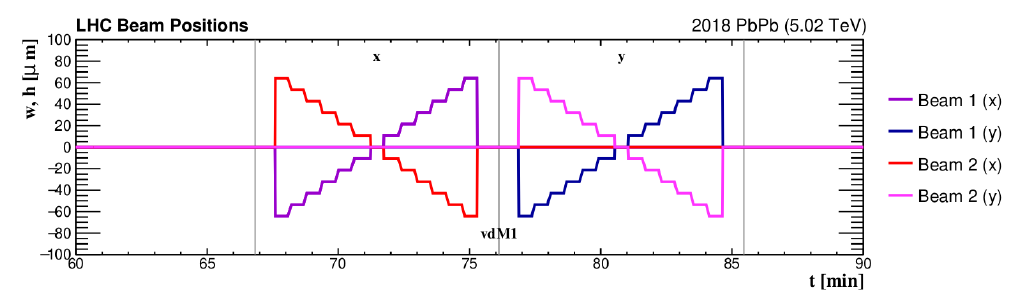
\includegraphics[width=\textwidth]{images/assets/vdm_scan_steps.png}
	\caption{Nominal LHC beam positions displaying the van der Meer scan sequence first in $x$-axis and then in $y$-axis (from \textit{Ref.} \cite{Saariokari:2826125}).}
	\label{fig:vdm_scan_steps}
\end{figure}


% \subsection{Experiment Conditions and Corrective Procedures}

% A vdM scan is conducted under experimental conditions that allow for the measurement of the visible cross-section with the best precision. These conditions include smaller beam intensities, which minimize the effect of MIB and reduce non-linearity effects due to high pileup, well-separated bunches, which minimize afterglow effects where the signal from the previous bunch crossing spills over into the current one, among others \cite{GRAFSTROM201597}. In addition to these optimized experimental conditions, a series of offline corrections are performed to ensure the required level of precision. Such corrections include:

% \begin{itemize}
%     \item Beam current currections: A multitude of different systems measure and monitor the beam conditions during the entire fill in order to allow for offline correction like the removal of non intend charges.
%     \item Background corrections: Background signal, be it beam-induced, detector noise or machine-induced, is typically present in the raw recorded rates. These additional contrinutions are removed.
%     \item Beam Effects: The electromagnetic interaction between the 2 LHC beams results in a disturbance in the nominal beam separation and shapes which effects the calibration measurement. These effects are taken into account and correcti for in the analysis.
%     \item Orbit Drift: During the vdM fill, the nominal position of the LHC beams may shift resulting. These effects are measured by Beam Position Monitors (BPM) that later provide information on how to correct the nominal beam separations.
%     \item Length Scale: The operational displacement of the LHC beams is done with a pair of steering dipoles located on either side of the IP. These displacements come with an associated uncertainty due to effects as magnet hysteresis or lattice imperfection \cite{Persson:2750277}. These uncertainties are also corrected.
%     \item XY Factorization: The vdM method works under the assumption that the tranvese particle distribution are independent in each direction, and therefore factorizable. If this assumption is not true, the calculated value for $A_{eff}$ will be biased. Studies are conducted to understand the magnitude of this bias and correct it.
% \end{itemize}

% A more detailed explanation of these corrections, as well as their impact on the measured calibration, will be given in \autoref{sec:analysis_of_vdm_data}.

\subsection{Experiment Conditions and Corrective Procedures}

A vdM scan is conducted under experimental conditions that allow for the measurement of the visible cross-section with the highest precision. These conditions include smaller beam intensities, which minimize the effect of MIB and reduce non-linearity effects due to high pileup, and well-separated bunches, which minimize afterglow effects where the signal from the previous bunch crossing spills over into the current one, among others \cite{GRAFSTROM201597}. In addition to these optimized experimental conditions, a series of offline corrections are performed to ensure the required level of precision. These corrections include:

\begin{itemize}
    \item \textbf{Beam current corrections:} Various systems measure and monitor the beam conditions throughout the entire fill to enable offline corrections, such as the removal of unintended charges.
    \item \textbf{Background corrections:} Background signals, whether beam-induced, detector noise, or machine-induced, are typically present in the raw recorded rates. These additional contributions are removed.
    \item \textbf{Beam effects:} The electromagnetic interaction between the two LHC beams causes disturbances in the nominal beam separation and shapes, affecting the calibration measurement. These effects are accounted for and corrected in the analysis.
    \item \textbf{Orbit drift:} During the vdM fill, the nominal position of the LHC beams may shift. These shifts are measured by Beam Position Monitors (BPM), which provide information to correct the nominal beam separations.
    \item \textbf{Length scale:} The operational displacement of the LHC beams is achieved using a pair of steering dipoles located on either side of the IP. These displacements come with associated uncertainties due to effects such as magnet hysteresis or lattice imperfections \cite{Persson:2750277}. These uncertainties are corrected.
    \item \textbf{XY factorization:} The vdM method assumes that the transverse particle distributions are independent in each direction and therefore factorizable. If this assumption is not true, the calculated value for \(A_{eff}\) will be biased. Studies are conducted to understand the magnitude of this bias and correct it.
\end{itemize}

A more detailed explanation of these corrections, as well as their impact on the measured calibration, will be provided in \autoref{sec:analysis_of_vdm_data}.


% \subsection{Extrapolation of vdM Calibration}

% The experimental conditions in which a vdM fill is performed, as well as all the extra corrections that are applied to the collected data, ensure a cross-section measurement with high precision and accuracy. However, the experiment conditions that allow for the most optimal probing of the SM, physics conditions, introduce a number of effects that affect the calibration for our luminometers. It is then necessary to extrapolate the results obtained during a vdM fill in order to correctly calibrate the luminosity measured in physics conditions.

% Physics conditions are tailored towards obtaining the largest ammount of data possible. This includes higher bunch populations compared to vdM and more colliding bunches, all of which increase the ammount of colliding particles. These conditions bring about two classes of effects on our luminometers:

% \begin{itemize}
%     \item Efficiency effects: Prolonged exposure to radation in the LHC cavern detiorates the luminometers to the point where they become less efficient. These effects are seen as a decrease in their reported luminosity throughout the data taking year.
%     \item Non linearity effects: The varying experimental conditions can have an effect on the reported luminosity of our detectors, as was already stated in \autoref{subsec:luminosity_detectors}. While some of these effects have their own corrective procedure, like out-of-time pileup \cite{Sirunyan:2759951}, others are corrected empirically.
% \end{itemize}

% In order to account for these 2 classes of effects, the measured luminosity goes through one final correction described by \autoref{eq:luminosity_integration}.

% \begin{equation}
%     \centering
%     \mathcal{L} = \frac{f_{rev} \cdot \mu}{\sigma_{vis} \cdot \epsilon} - \alpha \left( \frac{f_{rev} \cdot \mu}{\sigma_{vis} \cdot \epsilon} \right)^{2}
%     \label{eq:luminosity_integration}
% \end{equation}

% As can be seen, 2 new parameters have been introduced. $\epsilon$ is the parameter that corrects for losses in efficiency in the detector throughout the year. To obtain these factors mini vdM-like scans, called emittance scans, are performed. These scans allow for the measurement of the visible cross-section with the same vdM method, although with less precision, which allows for the analysis of the evolution of this quanity across the year. A figure of merit (FOM) is then calculated as

% \begin{equation}
%     \centering
%     \text{FOM} = \frac{\sigma^{\text{vdM}}_{vis}}{\sigma^{\text{emit}}_{vis}}
%     \label{eq:figure_of_merit}
% \end{equation}

% where $\sigma^{\text{vdM}}_{vis}$ is the visible cross-section measured in vdM conditions and $\sigma^{\text{emit}}_{vis}$ is the one measured in emittance scans during physics conditions. These FOM values are calculated for every emittance scan across the year and are the values given to $\epsilon$ in \autoref{eq:luminosity_integration}. This procedure allows for the extrapolation of the vdM calibration to the rest of the physics fills.

% The second new parameter is $\alpha$ and it is used to correct for any non linearity in the luminometers in an emperical way. Non linearity is defined as any non linear response to changes in the experimental conditions. \autoref{fig:non_linearity_diagram} ilustrates the response of a theoretical linear detector, a detector with positive non linearity and a detector with negative non linearity.

% % \begin{figure}[h]
% % 	\centering
% % 	\includegraphics[width=0.7\textwidth]{images/assets/non_linearity_diagram.pdf}
% % 	\caption{Ilustration of non linearity effects on measured SBIL as a function of the true SBIL. The two marked regions serve the purpose of illustrating the effects of extrapolating from vdM to physics conditions.}
% % 	\label{fig:non_linearity_diagram}
% % \end{figure}

% \begin{figure}[h]
% 	\centering
% 	\makebox[\textwidth][c]{%
% 		\begin{minipage}[b]{0.5\textwidth}
% 			\centering
%             \includegraphics[width=\textwidth]{images/assets/non_linearity_diagram.pdf}
%             \subcaption{}
%             \label{fig:non_linearity_diagram}
% 		\end{minipage}
% 		\begin{minipage}[b]{0.5\textwidth}
% 			\centering
%             \includegraphics[width=\textwidth]{images/assets/non_linearity_method.pdf}
%             \subcaption{}
%             \label{fig:non_linearity_method}
% 		\end{minipage}
% 	}
% 	\caption{(a) Ilustration of non linearity effects on measured SBIL as a function of the true SBIL. The two marked regions serve the purpose of illustrating the effects of extrapolating from vdM to physics conditions. (b) Non linearity extracted for the PLT and BCM1F detectors with respect to DT for fill 9029. Each data point is the ratio of the luminosities averaged over 15 lumi sections.}
% \end{figure}

% The reasons for a detector to have a positive or negative non-linear response differ:

% \begin{itemize}
%     \item PLT has consistently reported signs of suffering from positive non linearity. This mostly comes from the fact that at higher pileup, the probability of a tripple coincidence event occuring accidentally increases, which provoques overcounting.
%     \item HFOC suffers from zero starvation effect and, as explained in \autoref{subsec:zero-counting} this leads to an underestimation of the measured rates which is categorized as a negative non linearity.
%     \item BCM1F, with the VME backend system, has a tendency to undercount at high pileup do to an increasing chance of simultaneous hits being registered as just one hit which lowers the measured rates.
% \end{itemize}

% Correcting for non linearity is challenging due to the lack of a perfectly linear reference detector, which prevents an obsolute measurement of non linearity. Instead, a reference detector, that is assumed to be linear, is used. In this method, a linear fit is performed to the ratio between a luminomter and this reference detector as a function of SBIL. \autoref{fig:non_linearity_method} ilustrates this method applied to PLT and BCM1F while using DT as the reference.

% % \begin{figure}[h]
% %     \centering
% %     \includegraphics[width=0.7\textwidth]{images/assets/non_linearity_method.pdf}
% %     \caption{Non linearity extracted for the PLT and BCM1F detectors with respect to DT for fill 9029. Each data point is the ratio of the luminosities averaged over 15 lumi sections.}
% %     \label{fig:non_linearity_method}
% % \end{figure}

% The slope extracted from the fit is then used as the value of $\alpha$ in \autoref{eq:luminosity_integration}. Unlike the efficiency correctoins, $\epsilon$, the non linearity corrections are done at the expense of introducing some degree of correlation between the corrected detector and the reference. For this reason, and in order to keep the luminometers as independent as possible, the slopes are only extracted for a few fills with high sbil range throughtout the year.


\subsection{Extrapolation of vdM Calibration}

The experimental conditions in which a vdM fill is performed, as well as all the extra corrections applied to the collected data, ensure a cross-section measurement with high precision and accuracy. However, the experimental conditions optimal for probing the Standard Model, known as physics conditions, introduce several effects that impact the calibration of our luminometers. Therefore, it is necessary to extrapolate the results obtained during a vdM fill to correctly calibrate the luminosity measured under physics conditions.

Physics conditions are tailored to obtaining the largest amount of data possible. This includes higher bunch populations compared to vdM fills and more colliding bunches, all of which increase the number of colliding particles. These conditions bring about two classes of effects on our luminometers:

\begin{itemize}
    \item \textbf{Efficiency effects:} Prolonged exposure to radiation in the LHC cavern deteriorates the luminometers, making them less efficient. These effects manifest as a decrease in the reported luminosity throughout the data-taking year.
    \item \textbf{Non-linearity effects:} Varying experimental conditions can affect the reported luminosity of our detectors, as mentioned in \autoref{subsec:luminosity_detectors}. While some of these effects have their own corrective procedures, such as out-of-time pileup \cite{Sirunyan:2759951}, others are corrected empirically.
\end{itemize}

To account for these two classes of effects, the measured luminosity undergoes a final correction described by \autoref{eq:luminosity_integration}.

\begin{equation}
    \centering
    \mathcal{L} = \frac{f_{rev} \cdot \mu}{\sigma_{vis} \cdot \epsilon} - \alpha \left( \frac{f_{rev} \cdot \mu}{\sigma_{vis} \cdot \epsilon} \right)^{2}
    \label{eq:luminosity_integration}
\end{equation}

Two new parameters have been introduced. \(\epsilon\) is the parameter that corrects for losses in detector efficiency throughout the year. To obtain these factors, mini vdM-like scans, called emittance scans, are performed. These scans measure the visible cross-section using the same vdM method, albeit with less precision, allowing for the analysis of the evolution of this quantity over the year. A figure of merit (FOM) is then calculated as:

\begin{equation}
    \centering
    \text{FOM} = \frac{\sigma^{\text{vdM}}_{vis}}{\sigma^{\text{emit}}_{vis}}
    \label{eq:figure_of_merit}
\end{equation}

where \(\sigma^{\text{vdM}}_{vis}\) is the visible cross-section measured under vdM conditions, and \(\sigma^{\text{emit}}_{vis}\) is the one measured during emittance scans under physics conditions. These FOM values are calculated for every emittance scan throughout the year and are assigned to \(\epsilon\) in \autoref{eq:luminosity_integration}. This procedure allows for the extrapolation of the vdM calibration to the rest of the physics fills.

The second new parameter is \(\alpha\), which corrects for any non-linearity in the luminometers empirically. Non-linearity is defined as any non-linear response to changes in experimental conditions. \autoref{fig:non_linearity_diagram} illustrates the response of a theoretical linear detector, a detector with positive non-linearity, and a detector with negative non-linearity.

\begin{figure}[h]
	\centering
	\makebox[\textwidth][c]{%
		\begin{minipage}[b]{0.5\textwidth}
			\centering
            \includegraphics[width=\textwidth]{images/assets/non_linearity_diagram.pdf}
            \subcaption{}
            \label{fig:non_linearity_diagram}
		\end{minipage}
		\begin{minipage}[b]{0.5\textwidth}
			\centering
            \includegraphics[width=\textwidth]{images/assets/non_linearity_method.pdf}
            \subcaption{}
            \label{fig:non_linearity_method}
		\end{minipage}
	}
	\caption{(a) Illustration of non-linearity effects on measured SBIL as a function of the true SBIL. The two marked regions illustrate the effects of extrapolating from vdM to physics conditions. (b) Non-linearity extracted for the PLT and BCM1F detectors with respect to DT for fill 9029. Each data point is the ratio of the luminosities averaged over 15 lumi sections.}
\end{figure}

The reasons for a detector to have a positive or negative non-linear response vary:

\begin{itemize}
    \item PLT has consistently shown signs of positive non-linearity, mainly due to the increased probability of accidental triple coincidence events at higher pileup, leading to overcounting.
    \item HFOC suffers from the zero starvation effect, as explained in \autoref{subsec:zero-counting}, leading to an underestimation of the measured rates, categorized as negative non-linearity.
    \item BCM1F, with the VME backend system, tends to undercount at high pileup due to the increasing chance of simultaneous hits being registered as a single hit, lowering the measured rates.
\end{itemize}

Correcting for non-linearity is challenging due to the lack of a perfectly linear reference detector, which prevents an absolute measurement of non-linearity. Instead, a reference detector assumed to be linear is used. In this method, a linear fit is performed on the ratio between a luminometer and this reference detector as a function of SBIL. \autoref{fig:non_linearity_method} illustrates this method applied to PLT and BCM1F, using DT as the reference.

The slope extracted from the fit is then used as the value of \(\alpha\) in \autoref{eq:luminosity_integration}. Unlike the efficiency corrections (\(\epsilon\)), the non-linearity corrections are done at the expense of introducing some degree of correlation between the corrected detector and the reference. To keep the luminometers as independent as possible, the slopes are extracted for only a few fills with a high SBIL range throughout the year.

\todo{Brief paragraph stating that specialized vdM conditions, the series of corrections we apply to vdm data and the extrapolation to physics conditions all contribute to the challenge of accuratly measuring luminosity at hadron colliders like the LHC.}

% \subsection{Additional scans}

% Other kinds of scans, besides the vdM scan, are also performed at the vdM fill. These other scans are done in order to provide specific insights on the various experimental conditions during the vdM fill:

% \begin{itemize}
%     \item Super Separation scans (ss): These scans are done by maximaly separating the beams in the LHC. This allowsfor an accurate measurement of the brackground signal for each luminometer.
%     \item Beam Imaging scans (bi): In these scans one of the beams is kept fixed in its nominal head on position while the other is scanned. They are used in the beam-imaging method \cite{Klute_2017} that is used in XY factorization analysis. A visible cross-section is also extracted from these scans as it is done to VdM scans.
%     \item Diagonal scans (diag): These scans are vdM scans done at distinct angles. Different variations like +45-45, +30-60 and +60-30 are used to allow the fitting to happen over different regions of the beam overlap. These scans are aslo used in XY factorization studies.
%     \item Offset scans (off): These have the same motion as in vdM scans only one of the beams is not in the nominal head on position. These scans are used in beam shape studies to determine the XY factorization bias.
%     \item Variable/Constant Length Scale scans (vLS, cLS): These scans are used to calibrate the distance by which the steering magnets displace the beams.
% \end{itemize}

% Each scan is separatly recorded and analysed offline. After due analysis, the corrective procedures that have been determined from each of these special scans are applied during the vdM scan analysis in order to correct the extracted detector calibration. In principle, these corrections affect every luminomenter in a similar fashion.

\subsection{Additional Scans}

In addition to the VdM scan, other types of scans are performed during the VdM fill to provide specific insights into the various experimental conditions:

\begin{itemize}
    \item \textbf{Super Separation scans (ss):} These scans involve maximally separating the beams in the LHC, allowing for an accurate measurement of the background signal for each luminometer.
    \item \textbf{Beam Imaging scans (bi):} In these scans, one beam is kept fixed in its nominal head-on position while the other beam is scanned. They are used in the beam-imaging method \cite{Klute_2017}, which is employed in XY factorization analysis. A visible cross-section is also extracted from these scans, similar to VdM scans.
    \item \textbf{Diagonal scans (diag):} These are VdM scans performed at distinct angles, such as +45/-45, +30/-60, and +60/-30. They allow the fitting to occur over different regions of the beam overlap and are used in XY factorization studies.
    \item \textbf{Offset scans (off):} These scans have the same motion as VdM scans, but one of the beams is not in the nominal head-on position. They are used in beam shape studies to determine the XY factorization bias.
    \item \textbf{Variable/Constant Length Scale scans (vLS, cLS):} These scans are used to calibrate the distance by which the steering magnets displace the beams.
\end{itemize}

Each scan is separately recorded and analyzed offline. After thorough analysis, the corrective procedures determined from each of these special scans are applied during the VdM scan analysis to correct the extracted detector calibration. In principle, these corrections affect every luminometer in a similar fashion.

\chapter{The problem and its challenges}

The problem and its challenges.

\section{Images}
Example of inserting an image as displayed text,
\begin{center}
	
\includegraphics[width=0.1\textwidth]{images/UM.jpg}
\end{center}

\begin{wrapfigure}{r}{0.15\textwidth}	
	
\includegraphics[width=0.1\textwidth]{images/UM.jpg}
\end{wrapfigure}
\noindent --- wrapped into the text,
bla-bla bla-bla bla-bla bla-bla bla-bla bla-bla bla-bla bla-bla bla-bla bla-bla
bla-bla bla-bla bla-bla bla-bla bla-bla bla-bla bla-bla bla-bla bla-bla bla-bla
bla-bla bla-bla bla-bla bla-bla bla-bla bla-bla bla-bla bla-bla bla-bla bla-bla
bla-bla bla-bla bla-bla bla-bla bla-bla bla-bla bla-bla bla-bla bla-bla bla-bla
bla-bla bla-bla bla-bla bla-bla bla-bla bla-bla bla-bla bla-bla bla-bla bla-bla bla-bla bla-bla bla-bla bla-bla
bla-bla bla-bla bla-bla bla-bla bla-bla bla-bla bla-bla bla-bla bla-bla bla-bla bla-bla bla-bla bla-bla bla-bla

\noindent --- or as a floating body.
\begin{figure}
\begin{center}
	
\includegraphics[width=0.25\textwidth]{images/UM.jpg}
\end{center}
\caption{Caption}
\end{figure}

\chapter{Contribution}

Main result(s) and their scientific evidence

\section{Introduction}

\section{Summary}
\chapter{Analysis Software}

The analysis of vdM data, along with the application of stability and linearity corrections, is carried out using two distinct frameworks, each playing a crucial role in ensuring the accuracy and reliability of the results.

The vdM Framework \cite{VdMFramework} is employed to execute all the corrections and fits detailed in \autoref{ch:2023_luminosity_calibration}. This tool is vital for managing the complex data processing required during the vdM scans, enabling precise calibration and adjustment of the luminometers. My contributions to the development and enhancement of this framework are discussed in \autoref{sec:the_vdM_framework}.

For integration corrections, the BRIL work suite (b' database. To query this database, and obtain the corrected datarilws) \cite{xie_bril} is utilized. This suite takes on the critical task of applying the final layer of luminosity corrections, as well as distributing the results to other CMS groups. The specific program responsible for these corrections is called brilcalc. The inner workings, limitations, developed alternatives, and my contributions to the improvement of this program are detailed in \autoref{sec:the_bril_work_suite}.

\section{The vdM Framework}
\label{sec:the_vdM_framework}

The vdM Framework (vdMFw) is the analysis software used by CMS to perform luminosity calibration measurements for all luminometers with per-bunch granularity. First commissioned in 2015, it has been continuously improved in line with the collaboration’s growing understanding of the systematics discussed in \autoref{ch:2023_luminosity_calibration}. Today, it serves as the primary framework for analyzing vdM scans, applying data corrections, and tracking luminometer operational conditions through emittance scan analysis throughout the year.

\subsection{Flow of the Analysis}

The flow of analysis in the vdMFw, outlined in \autoref{fig:vdm_fw_flowchart}, begins with user-provided input. This input can be categorized into two types: the data to be analyzed and the user specifications that dictate how the analysis should be conducted.

\begin{figure}[!htb]
	\centering
	\makebox[\textwidth]{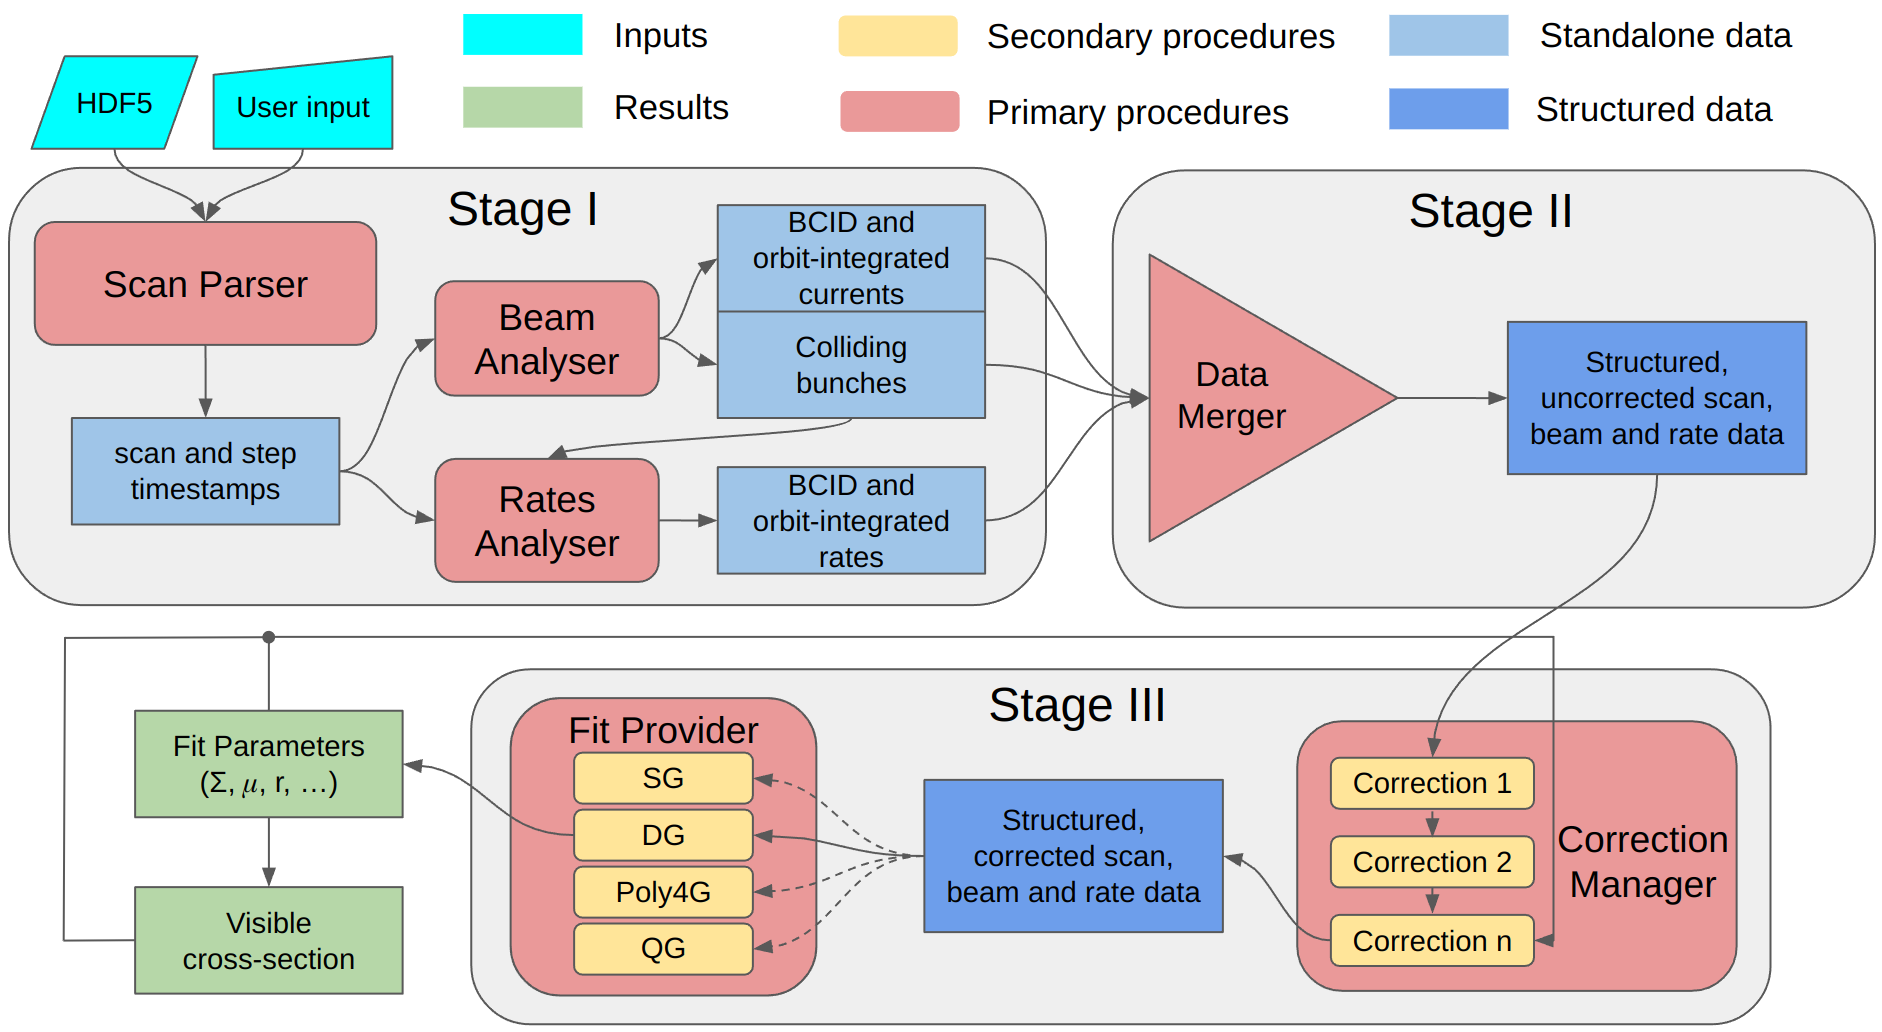
\includegraphics[width=0.7\paperwidth]{images/assets/vdm_fw_flowchart.png}}
	\caption{Overview of the flow of the analysis in the vdMFw.}
	\label{fig:vdm_fw_flowchart}
\end{figure}

The data is provided in Hierarchical Data Format 5 (HDF5) \cite{koranne2011hierarchical}, which includes scan, luminometer, and beam information for a particular period of time:
\begin{itemize}
	\item \textbf{Scan data}: Includes beam separation information, which is used to extract the beginning and end timestamps of each scan step.
	\item \textbf{Beam data}: Contains the beam currents, both per-orbit and per-bunch, saved in the beam table of the input file.
	\item \textbf{Luminometer data}: Stores the counts for every luminometer in operation during the time period associated with the input file.
\end{itemize}
The user can specify the following input parameters:
\begin{itemize}
	\item Which luminometer data to analyse. The results of the analysis will correspond to the calibration constant for this luminometer.
	\item The fit function to be used for the bunch overlap shapes.
	\item The corrections to be applied. Some corrections are derived from the input data file, while others require external inputs from parallel analyses.
	\item Optionally, the user may provide a \textit{ratefile}, also in HDF5 format, which contains only luminometer rates. This is useful when the original luminometer data is corrupted, non-existent, or when some offline correction has been applied to the original data.
\end{itemize}
Additionally, there is a user configuration file where further details can be adjusted.

The first stage of the analysis involves the preparation of the individual inputs that go into the fitting procedure, such as the beam separations and the rates normalized to the beam currents. The Scan Parser extracts the timestamps associated with each scan step and feeds them into the subsequent blocks. The Beam Analyser identifies the colliding bunches and computes the beam currents. At this stage, the beam current corrections explained in \autoref{subsec:beam_current_measurement} are applied. The colliding bunch indices are then passed to the Rates Analyser, where the luminometer rates are calculated.

The data processed in the previous stage is passed to Stage II. This stage consolidates all the pieces of information into a structured format to facilitate the application of any corrections and fits that follow.

Lastly, Stage III applies all the requested corrective procedures, and finishes in a fit to the corrected data, which provides the fit parameters used in calculating the detector calibration constants. While all corrections are done sequentially, some require outputs from previous corrections, hence the backward connector from the results to the beginning of this stage. The analysis concludes with all the results, both intermediate and final, being saved to files for later inspection.

\subsection{Input/Output bottleneck}
\label{subsec:io_bottleneck}

The vdMFw is executed multiple times throughout the year, particularly during emittance scans and vdM fills, where numerous corrections must be applied. Additionally, the process of adjusting the calibrations and ensuring detector stability is highly iterative, requiring the analysis to be run repeatedly until the results achieve the desired precision. Consequently, efforts have been made to enhance the software's performance.

To identify the primary bottlenecks within the framework, an initial profiling was conducted on input HDF5 files corresponding to vdM scans. These files were chosen because they undergo the complete correction pipeline, providing a comprehensive diagnosis of performance issues.

The profiling was performed on a system with the following specifications: x86\_64 architecture, equipped with 32 CPUs, each with 2 threads per core, distributed across 8 cores per socket, and 2 sockets in total. The CPUs operate at a base frequency of 1.0 GHz, with a maximum frequency of 3.5 GHz, supported by 64 GB of RAM and an L3 cache of 11 MB.

The results of the profiling are presented in \autoref{tab:profiling_results}, which highlights the time spent in each stage of the analysis process.

\begin{table}[!htb]
	\centering
	\caption[Initial vdMFw profiling results]{Initial profiling results shown separately for the procedures in Stage I and combined for Stages II and III. The times correspond to an average of 50 runs where the full analysis pipeline was executed.}
	\begin{tabular}{|l|c|c|}
		\hline
		\textbf{Procedure} & \textbf{Time [s]} & \textbf{\% of total program} \\
		\hline
		Scan Parser        & 0.34 $\pm$ 0.01   & 0.27                         \\
		Beam Analyser      & 37.11 $\pm$ 0.65  & 29.60                        \\
		Rate Analyser      & 57.85 $\pm$ 1.18  & 46.15                        \\
		Stage II + III     & 30.06 $\pm$ 0.57  & 23.98                        \\
		\hline
	\end{tabular}
	\label{tab:profiling_results}
\end{table}

As shown in \autoref{tab:profiling_results}, the most significant bottlenecks were identified in the Beam Analyser and Rate Analyser procedures, which together account for over 75\% of the total execution time. This result was unexpected, as the bulk of the framework’s workload was anticipated to revolve around data corrections and fitting procedures.

Upon closer inspection of the code within these two time-consuming procedures, the reason for their substantial execution time became apparent. To generate the expected outputs, these procedures need to read relevant data from the input HDF5 files. In the original implementation, the reading process occurred for every scan step, as follows:

\begin{enumerate}
	\item Read the entire rate (or beam) table\footnote{HDF5 files are organized in folder-like structures. The \textit{tables} are analogous to files in this structure, and in BRIL's case, each table contains specific data related to the LHC.} from the HDF5 file into memory.
	\item Filter for the timestamps corresponding to the current scan step.
\end{enumerate}

Reading the entire table content each time is computationally expensive, as the amount of data to be read can consume a significant portion of the execution time. The profiling mentioned above was conducted using data files already filtered by the time period during which the scan was performed, resulting in smaller data files (approximately 23 MB). However, when the same profiling was run with an optional \textit{ratefile} of 1631 MB in memory, the execution time of the Rate Analyser procedure increased dramatically from 57.85 seconds to 446.34 seconds, clearly indicating an Input/Output-related bottleneck.

To improve these execution times, the following optimizations were implemented:

\begin{itemize}
	\item The corresponding rate (or beam) table is now read only once before computing the per-step results.
	\item Instead of loading the entire table content into memory, which could lead to crashes if the data size exceeds the available RAM + SWAP\footnote{SWAP space is a portion of the hard drive designated to act as virtual memory when the physical RAM is fully utilized. It helps prevent crashes by providing additional memory space, though it is much slower than actual RAM.} space, a first pass is performed to gather all the entries that fall within any scan step.
	\item Only the relevant entries identified in the previous step are then read.
\end{itemize}

These changes led to the improved profiling results shown in \autoref{tab:profiling_results_2}:

\begin{table}[!htb]
	\centering
	\caption[vdMfw profiling results after performance improvements]{Profiling results after implementing the optimizations in the analyser procedures. The results show significant improvements in both procedures. The bulk of the framework (Stages II and III) now accounts for 95\% of the total program execution time, and the overall program speedup was approximately 4 times.}
	\begin{tabular}{|l|c|c|}
		\hline
		\textbf{Procedure} & \textbf{Time [s]} & \textbf{\% of total program} \\
		\hline
		Scan Parser        & 0.35 $\pm$ 0.02   & 1.08                         \\
		Beam Analyser      & 0.90 $\pm$ 0.11   & 2.80                         \\
		Rate Analyser      & 0.36 $\pm$ 0.02   & 1.11                         \\
		Stage II + III     & 30.46 $\pm$ 0.54  & 95.01                        \\
		\hline
	\end{tabular}
	\label{tab:profiling_results_2}
\end{table}

When running the profiling on the same larger \textit{ratefile} as before, the average execution time was reduced to $7.9 \pm 0.22$ seconds, representing a speedup of approximately 56 times compared to the original implementation.

\subsection{Online vdM Analysis}

An important aspect of analyzing LHC scans is the ability to process data immediately after a scan is completed, a process referred to as online analysis. Quick feedback from the framework allows for the possibility of repeating scans if any issues are identified during their execution. This capability is especially critical during vdM fills, motivating the enhancements made to this workflow.

\begin{figure}[!htb]
	\centering
	\makebox[\textwidth]{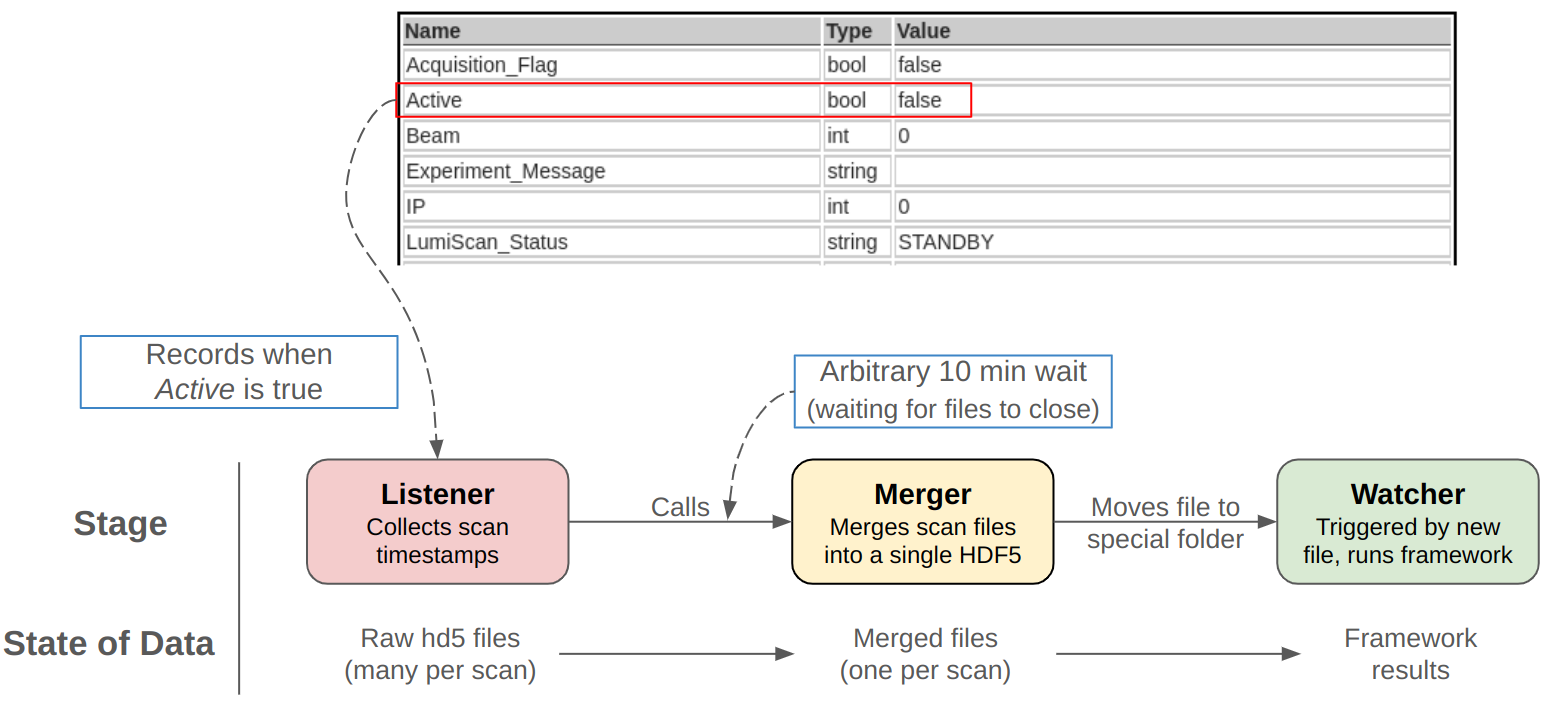
\includegraphics[width=0.7\paperwidth]{images/assets/online_analysis_workflow.png}}
	\caption{Workflow of the online analysis.}
	\label{fig:online_analysis_workflow}
\end{figure}

The workflow, illustrated in \autoref{fig:online_analysis_workflow}, begins with the Listener stage. This component constantly queries the xDAQ data acquisition system \cite{Brigljevic:845273} for the \textit{Active} variable, which is set to true while a scan is ongoing at the CMS IP. During these periods, two independent processes are at work:

\begin{itemize}
	\item \textbf{BRIL Data Acquisition System (BRILDAQ)}: BRILDAQ, built on top of xDAQ, is the data transfer system used by all BRIL systems. It is configured to save extra HDF5 files to a specific destination while \textit{Active} is set to true. These files are smaller and each contains data for a portion of the entire scan.
	\item \textbf{Scan Listener}: The Listener, a separate process also built using xDAQ, continuously monitors the \textit{Active} variable and records the timestamps corresponding to the beginning and end of a scan (when \textit{Active} changes from false to true and from true to false).
\end{itemize}

Once a scan is completed, the Listener passes the timestamp information to the Merger, which consolidates all files created within those timestamps. Since the two processes mentioned earlier operate independently, a safeguard in the form of a 10-minute wait time was implemented to protect against potential I/O errors. The output of the Merger is a single file containing data for the entire scan. This file is then moved to a designated folder monitored by the Watcher.

The Watcher is a filesystem event manager designed to trigger whenever a new file is created in a specific directory. Each trigger initiates the vdMFw to analyze that particular scan, applying multiple fits, corrections, and processing all online luminometers.

\subsection{Improving Wait Time in Merger}

The fixed waiting time in the Merger block is suboptimal. If the wait time is too short, it could lead to I/O problems, whereas if it is too long, it could delay the ability to repeat a scan, which is particularly critical during vdM fills.

To address this, an alternative approach was introduced in the Merger step that continuously polls the intermediate HDF5 files to check if they have been closed. This was implemented using the \textit{lsof} Linux utility, which provides a convenient API to determine which files are open by which processes. The implementation of this polling mechanism can be seen in \autoref{lst:merger_polling}.

During the 2024 vdM program, which started on May 16th, the time spent waiting for the files to close for all vdM and im scans was significantly shorter than the fixed 10-minute interval, as shown in \autoref{tab:time_waiting_2024}.

\begin{table}[!htb]
	\centering
	\caption{Time spent waiting for scan files to close in the Merger during the 2024 vdM fill.}
	\begin{tabular}{|c|c|c|c|c|c|c|c|c|}
		\hline
		\textbf{Scan}     & vdm1  & vdm2  & vdm3  & vdm4  & vdm5  & im1   & im2   & vdm6  \\
		\hline
		\textbf{Time [s]} & 27.97 & 24.53 & 25.04 & 26.69 & 32.79 & 18.29 & 19.19 & 27.25 \\
		\hline
	\end{tabular}
	\label{tab:time_waiting_2024}
\end{table}

Being the most time consuming stages of this workflow the wait time in the Merger and running the vdMFw, these improvements allow for a feedback time of approximately 1 min after a particular scan has finished, a significant improvement over the 10+ minutes it used to take previously.
 

\section{The BRIL Work Suite}
\label{sec:the_bril_work_suite}

The \textit{brilcalc} tool, part of the BRIL work suite, plays a critical role in providing other CMS groups with access to the most accurate and up-to-date luminosity data from BRIL. This section will first explain how \textit{brilcalc} operates, including the necessary special input files, before discussing the enhancements made to its usability and maintenance. Finally, a highly requested alternative to \textit{brilcalc} will be introduced, along with an analysis of its advantages and disadvantages.

\subsection{Normtags and Iovtags}

\begin{figure}[!htb]
	\centering
	\makebox[\textwidth]{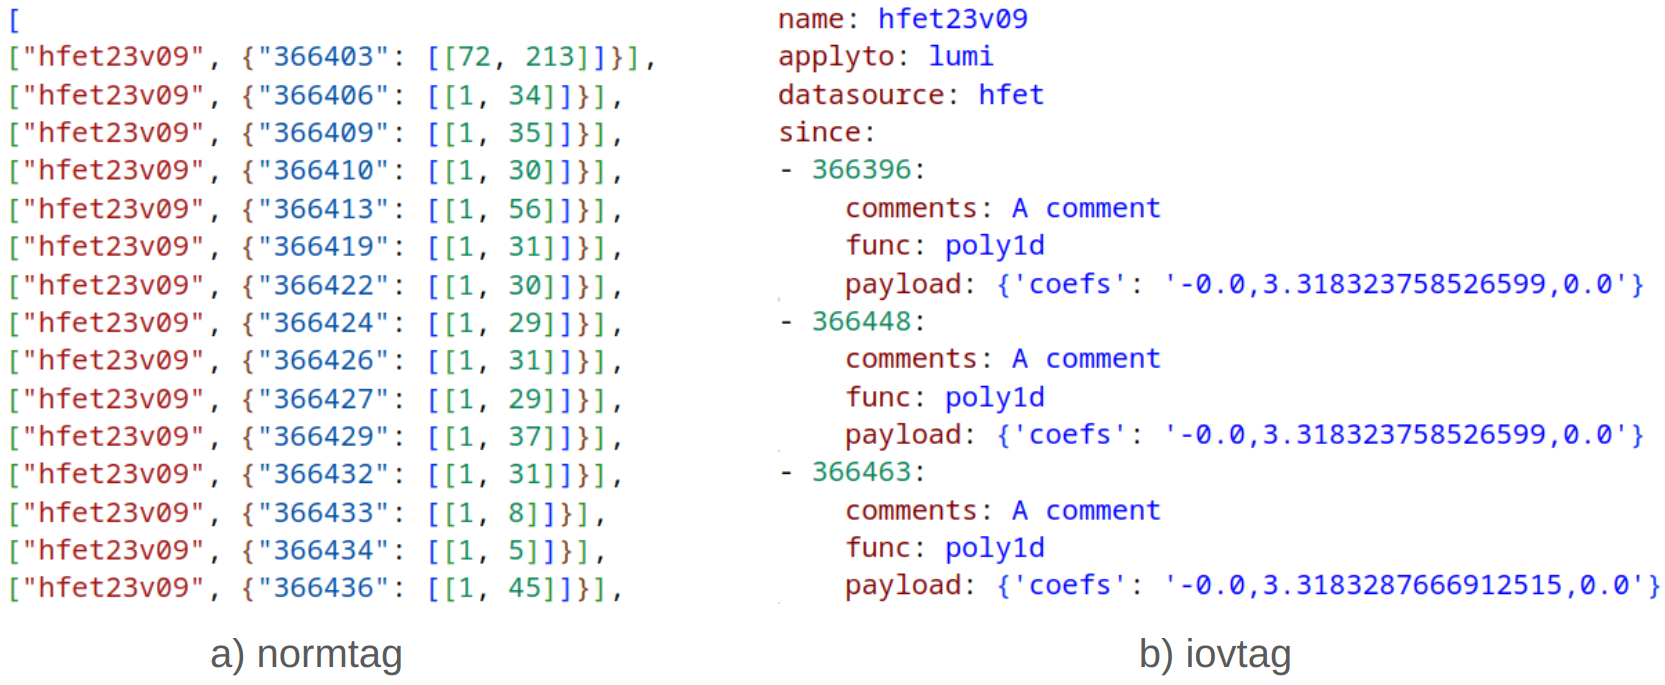
\includegraphics[width=0.7\paperwidth]{images/assets/normtag_iovtag.png}}
	\caption[Illustration of iovtag and normtag file structure]{a) Example of a Normtag file specifying LHC periods for queries in brilws' database. Each period is defined by a run number and a range of valid lumisections for that run. b) Example of an Iovtag file corresponding to the HFET luminometer, specifying correction functions and payload arguments for each run number at the beginning of a fill.}
	\label{fig:normtag_iovtag}
\end{figure}

Given the high data demands from both BRIL and other CMS groups, \textit{brilcalc} needs to efficiently retrieve luminosity results for any requested period. To meet this requirement, data initially stored in HDF5 files is loaded into the brilws database. \textit{Brilcalc} relies on two specific input files for querying the database: a \textit{normtag} and an \textit{iovtag} file. The \textit{normtag} file defines the LHC periods to be queried, while the \textit{iovtag} file specifies how to apply corrections to the data from those periods. The structure of these files is illustrated in \autoref{fig:normtag_iovtag}.

To interpret these files:
\begin{itemize}
	\item The first entry in the normtag specifies: For all lumisections in $[72, 213]$ of run 366403, use the iovtag hfet23v09.
	\item The first entry in the iovtag specifies: For all runs in $[366396, 366447]$, correct HFET's luminosity by applying the function \textit{poly1d} with the parameters \textit{\{'coefs': '-0.0,3.318323758526599,0.0'\}}.
\end{itemize}

The correction applied by the \textit{poly1d} function corresponds to the procedure explained in \autoref{subsec:extrapolation_of_vdM_calibration}. The \textit{coefs} field contains three comma-separated values that represent the coefficients of a second-degree polynomial in descending order. Since \textit{brilcalc} operates on rate data from the HDF5 files, the coefficients are derived using:

\begin{equation}
    \centering
    \mathcal{L} = \underbrace{C_0}_{\text{0th order}} + \underbrace{\frac{f_{rev}}{\sigma_{vis} \cdot \epsilon}}_{\text{1st order}} \mu + \underbrace{- \alpha \left( \frac{f_{rev}}{\sigma_{vis} \cdot \epsilon} \right)^{2}}_{\text{2nd order}} \mu^2
    \label{eq:brilcalc_poly1d}
\end{equation}

\subsection{Limitations}

Despite being the primary tool for obtaining the latest luminosity results, \textit{brilcalc} was not originally designed for iterative analysis processes. Each time a new version of HDF5 data for a specific luminometer is created, it must be uploaded to the database. This process is not only time-consuming, as only authorized maintainers can update the database, but it also poses a risk of contaminating the database with incorrect data since uploads are not automatically validated for accuracy.

There are also issues with the construction of iovtags. As shown in \autoref{fig:normtag_iovtag}b, the \textit{payload} parameter of iovtags is often not descriptive, requiring creators to add meaningful comments that help users interpret the values of $\sigma_{\text{vis}}$, $\epsilon$, and $\alpha$ that generated the \textit{coefs}.

Another significant problem is the lack of thorough validation for iovtags submitted to the database. The original system only checks the iovtag schema, not its content. Combined with minimal commenting, this can complicate the management of multiple iovtags across different systems and increase the difficulty of ensuring reproducibility of results.

\subsection{Enhancements to Iovtags}

The software responsible for applying corrections specified by \textit{iovtags} is built around a Python class containing various methods for implementing different types of luminosity corrections. For each correction, the specific method to be called is determined by the \textit{func} parameter within the \textit{iovtag}, and the method uses the corresponding \textit{payload} to compute the corrected luminosity. Below is a simplified version of the existing code:

\begin{lstlisting}
class LuminosityCorrector:
  def poly1d(self, database_input, payload):
    coefs_array = np.fromstring(payload["coefs"], dtype=np.float, sep=',')

    # Logic to fetch the rates and number of colliding bunches from the database
    rates = ...
    ncol = ...

    # Divide by ncol to get the SBIL
    return ncol * np.poly1d(rates / ncol, coefs_array[::-1])
\end{lstlisting}

The first enhancement to the iovtag workflow was to introduce a new set of payload parameters. A new function, \textit{poly1d2}, where "2" denotes version 2, was implemented as follows:

\begin{lstlisting}
def poly1d2(self, database_input, payload):
  # Logic to fetch the rates and number of colliding bunches from the database
  rates = ...
  ncol = ...

  lumi = (payload["frev"] * rates / ncol) / (payload["sigvis"] * payload["eff"])
  return payload["constant"] + lumi - payload["alpha"] * lumi**2
\end{lstlisting}

This alternative implementation provides several advantages:

% \begin{itemize}
%     \item When using \textit{poly1d2}, the payload values become transparent, allowing anyone with access to the \textit{iovtag} to see the individual components rather than just the final coefficients from \autoref{eq:brilcalc_poly1d}. This is demonstrated in the following example:

% 	\begin{lstlisting}[language=Yaml]
% - 366396:
%   comments: A comment
%   func: poly1d2
%   payload:
%     frev: 11245.5
%     sigvis: 3394.33
%     eff: 1.02
%     slope: 0.0
%     constant: 0.0
% 	\end{lstlisting}

%     \item The new format simplifies comparisons between different versions of \textit{iovtags} for the same system, as only the \textit{comments} and \textit{payload} values differ. In the previous format, users could only guess what caused differences in coefficients.

%     \item The payload arguments effectively document the \textit{iovtag}, reducing the reliance on comments, which can often be incorrect or outdated. This self-documentation increases the robustness of \textit{iovtags} over time, as the essential details are embedded within the parameters themselves.

%     \item Including the calculation components directly within the \textit{iovtag} centralizes the code, reducing the risk of errors when applying the formula described in \autoref{eq:brilcalc_poly1d}.
% \end{itemize}

This alternative implementation offers several advantages. Firstly, when using \textit{poly1d2}, the payload values become transparent, allowing anyone with access to the \textit{iovtag} to see the individual components rather than just the final coefficients from \autoref{eq:brilcalc_poly1d}. This is evident in the following example:

\begin{lstlisting}[language=Yaml]
- 366396:
    comments: A comment
    func: poly1d2
    payload:
        frev: 11245.5
        sigvis: 3394.33
        eff: 1.02
        slope: 0.0
        constant: 0.0
\end{lstlisting}

This new format simplifies comparisons between different versions of \textit{iovtags} for the same system, as only the \textit{comments} and \textit{payload} values differ, whereas in the previous format, users could only speculate about the reasons behind differences in coefficients. Moreover, the payload arguments effectively document the \textit{iovtag}, reducing reliance on comments, which can often be incorrect or outdated. This self-documentation makes \textit{iovtags} more robust over time, embedding essential details directly within the parameters themselves. Additionally, including the calculation components directly within the \textit{iovtag} centralizes the code, reducing the risk of errors when applying the formula described in \autoref{eq:brilcalc_poly1d}.

Although this new approach improves the readability of \textit{iovtags}, it does not fully address the lack of stable, up-to-date documentation for the parameters of each method within the corrector class, nor does it validate \textit{iovtags} upon upload. To address both issues while maintaining tight coupling with the source code, Python decorators were employed \cite{pep318}.

A decorator named \textit{register\_sanitizer} was used on all correction methods to document each \textit{payload} parameter. An example of decorating the \textit{poly1d2} method is shown below:

\begin{lstlisting}
@register_sanitizer(
  required_params=(
    ("frev", "LHC's revolution frequency."),
    ("sigvis", "Luminometer visible cross-section."),
    ("eff", "Efficiency factor applied to 'sigvis'."),
    ("alpha", "Slope extracted from a linear fit to sbil_1 / sbil_2 = a * sbil_2 + b."),
    ("constant", "0th degree coefficient of the 2nd-degree polynomial."),
  )
)
def poly1d2(self, database_input, payload):
  ...
\end{lstlisting}

This decorator ensures that the \textit{poly1d2} function checks for the presence of all required parameters in the \textit{iovtag} before executing. For methods requiring constraints on parameters, the decorator also accepts a \textit{validators} parameter, as shown below:

\begin{lstlisting}
@register_sanitizer(
  required_params=(
    ("frev", "LHC's revolution frequency."),
    ("sigvis", "Luminometer visible cross-section."),
    ("eff", "Efficiency factor applied to 'sigvis'."),
    ("alpha", "Slope extracted from a linear fit to sbil_1 / sbil_2 = a * sbil_2 + b."),
    ("intercept", "Intercept extracted from the linear fit."),
    ("constant", "0th degree coefficient of the 2nd-degree polynomial."),
  ),
  validators=(
    (lambda payload: not np.isclose(payload["alpha"], 0.0), "'alpha' parameter cannot be 0."),
  )
)
def another_method(self, database_input, payload):
  ...
\end{lstlisting}

In the implementation of this decorator (see \autoref{lst:register_sanitizer}), the attributes \textit{\_required\_params} and \textit{\_validators} are added to the function objects to differentiate them from other class attributes. A class decorator named \textit{collect\_sanitizers} is used as a metaclass \cite{pep3115}, which gathers all registered sanitizers into class attributes upon loading, as illustrated in \autoref{lst:collect_sanitizers}.

This setup allows the sanitizers to be used not only on already loaded iovtags but also on those requested for upload. The \textit{validate\_iovtag\_data} function, shown in \autoref{lst:validate_iovtag_data}, implements the validation logic and is called each time a new iovtag is to be uploaded.

All these modifications allow the users of brilws to be more certain of the contents of the \textit{iovtags} they use as well as prevents poluting the database with erroneous correctors.


% \subsection{An alternative to brilcalc}

% The most theckincally challenging aspect of luminosity analysis is managing the different data versions. Any experimental effect that was not dealt with during operations has to be corrected for in offline analysis in a process that is tipically reffered to as reprocessing. Every reprocessing, takes as input a particular version of the HDf5 data for a given system, or systems, and corrects for one or multiple systematics. The result, is a new set of HDF5 files with the added correction.

% In principle, every new set of HDF5 files would be checked to assert that the correction was correctly applied. However, the checking of the results often required that the files were first uploaded to brilws' database. This, apart from leading to potential polution of the data in the database, leads to an extra data version in the database. An alternative, capable of producing the same outputs as brilcalc from just HDF5 files, was hightly requested.

% The software solution, although separate from brilws, was developed to be compatible to brilws workflow. It asks users to provide a \textit{nomrtag} file as well as the path location of the HDF5 files to be corrected. The \textit{iovtags} refered in the \textit{nomrtag} have to exist in disk but do not need to be loaded onto any database. The final output of this tool is in the same as in brilcalc. This tool opens up the possibility to rigorously test the result of any reprocessing before deciding to share the data with the rest of CMS.

% Even though the output of both tools is the same, there are advantages to using each:

% \begin{itemize}
% 	\item This alternative leaves no doubt has to what version of the data is being analysed since a path to the datafiles must be provided.
% 	\item The alternative is considerably slower then the brilws implementation. This is because reading the data directly from disk is considerably slower than querying a database.
% 	\item Even though its slower, it is fast enough as to allow multiple iterations of the analysis. In fact, for 2023 the stability and non-linearity corrections for the BCM1F system benifited mostly from it as multiple versions of this analysis took place. 
% \end{itemize}

% In conclusion, this alternative is extremely usefull for doing actual analysis while brilcalc is now used as the production equivalent for the analysis results. 

\subsection{An Alternative to brilcalc}

One of the most technically challenging aspects of luminosity analysis is managing the different versions of data. Any experimental effect not addressed during operations must be corrected in offline analysis, a process commonly referred to as reprocessing. Each reprocessing step takes as input a specific version of the HDF5 data for a given system or set of systems and applies corrections for one or more systematic effects, resulting in a new set of HDF5 files with the added corrections.

Ideally, each new set of HDF5 files would be thoroughly checked to ensure that the corrections were properly applied. However, verifying the results often required that the files first be uploaded to the brilws database, which not only risked contaminating the database with incorrect data but also unnecessarily increased the number of data versions stored. Consequently, there was a high demand for an alternative tool capable of producing the same outputs as \textit{brilcalc} directly from HDF5 files without the need for database integration.

The proposed software solution, while separate from brilws, was designed to be compatible with the brilws workflow. It requires users to provide a \textit{normtag} file and specify the location of the HDF5 files to be analyzed. The \textit{iovtags} referenced in the \textit{normtag} must exist on disk but do not need to be loaded into any database. The final output of this tool matches the format produced by \textit{brilcalc}, enabling rigorous testing of any reprocessing results before deciding to share the data with the rest of the CMS.

Although both tools produce the same output, each has distinct advantages. The alternative tool provides absolute certainty regarding the version of the data being analyzed since users must specify the exact path to the data files. However, this alternative is significantly slower than the brilws implementation because reading data directly from disk is much slower than querying a database. Despite this slower speed, it is still fast enough to allow multiple iterations of analysis, making it particularly useful for 2023, where the stability and non-linearity corrections for the BCM1F system benefited greatly from this approach, as multiple reprocessing steps were required.

In conclusion, while this alternative tool proves invaluable for conducting detailed analyses, \textit{brilcalc} remains the preferred option for production-level results, offering a more streamlined and faster approach once the data is finalized.

\chapter{Conclusions and future work}
Conclusions and future work.

\section{Conclusions}

\section{Prospect for future work}
		

\renewcommand{\baselinestretch}{1}
\bibliographystyle{abbrv}
\bibliography{dissertation}
\printindex

% \appendix
% \renewcommand\chaptername{Appendix}

\chapter{Appendices}

\chapter{Listings}
	Should this be the case.

\pagestyle{empty}
\cleartoevenpage
\null
\thispagestyle{empty}
\pagecolor{PANTONECoolGray7C}
\afterpage{\nopagecolor}
\newpage

\begin{backcover}
\thispagestyle{empty}{~\vfill
\noindent
Place here information about funding, FCT project, etc. in which the work is framed. Leave empty otherwise.
\vfill ~}
\end{backcover}



\end{document}
